\chapter{Variation of Galaxy Radius \& Morphology With Environment: Beyond the Local Universe with Hyper Suprime-Cam} \label{chap:morph_den}


{\large \emph{Aritra Ghosh, C. Megan Urry, Meredith C. Powell, Rhythm Shimakawa, Daisuke Nagai}} 


\section{Introduction} \label{sec_c4:intro}

$\Lambda$CDM cosmological models predict that galaxies form early in denser environments, and undergo more dynamical effects (i.e., mergers, harassment) compared to their counterparts in less dense regions. Therefore, galaxy properties should reflect this environmental effect.

It has been shown (conclusively) that galaxy color/star formation rates are a function of local density, and there are multiple studies that have confirmed this using extensive wide-field surveys \citep[e.g.,][]{Kauffmann04, Blanton05, Tanaka05, baldly_06, Peng10, Wetzel12, Alpaslan15, Duarte18, Old20}.


\begin{table}[htbp]
    \centering
    \caption{Selected Previous Studies of Environmental Dependence  at $z > 0.2$ \label{tab_c4:lit_survey}}
    \begin{tabular}{cccLL}
    \hline
    \hline
    Reference & Redshift & Sample & Radius & Morphology\\
     & &  Size & Summary\textsuperscript{a} & Summary\textsuperscript{b} \\
    \hline
    \hline
    \citet{Siudek22} & 0.5 - 0.9 & $\sim 30,000$ & $+$ve correlation only for blue galaxies & - \\
    \hline
    \citet{Gu21} & 0.5 - 2.5 &  & No correlation & No correlation\\
    \hline
    \citet{Afonso19} & 0.8 - 0.9  & $\sim 500$ & $+ve$ correlation only for galaxies with $\log M/M_{\odot} > 11$ & $+ve$ correlation\\
    \hline
    \citet{Matharu19} & $\sim1$  & $\sim600$ & $-ve$ correlation & -\\
    \hline
    \citet{Chan18} & 1.39 - 1.61  & $\sim3000$& $-ve$ correlation & -\\
    (passive only) & &  & & \\
    \hline
    \citet{Kelkar15} & 0.4 - 0.8  & $\sim400$ & No correlation & -\\
    \hline
    \citet{Bassett13} & $\sim1.6$  & $\sim 433$ & $+ve$ correlation for quiescent galaxies& $-ve$ correlation for quiescent galaxies\\
    \hline
    \citet{Huertas-Company13}  & 0.2 - 1.0 & $\sim700$ & No correlation & -\\
    (passive only) & &  & & \\
    \hline
    \citet{Lani13} & 1.0 - 2.0 & $\sim96,000$ & $+ve$ correlation only for passive galaxies & N/A\\
    \hline
    \citet{Cooper12} & 0.4 - 1.2  & $\sim600$ & $+ve$ correlation for early-type galaxies & -\\
    \hline
    \citet{Tasca09} & 0.1 - 1.2 &  $\sim10,000$ & - & Correlation observed\\
    \hline
    \hline
    \multicolumn{5}{p{0.95\textwidth}}{\vskip 0.01cm \small \textsuperscript{a} $+ve$ correlation refers to larger galaxies being present in denser environments } \\
    \multicolumn{5}{p{0.95\textwidth}}{\small \textsuperscript{b} $+ve$ correlation refers to galaxies with larger \sersic index or bulge-to-total light ratio being present in denser environments} \\
    \end{tabular}
\end{table}

However, the variation of galaxy size and morphology with environment is not well-established at all. Beyond the local universe ($z > 0.2$), different studies have reported conflicting results; as summarized in Table \ref{tab_c4:lit_survey}. While some studies have reported +ve correlation of radius with the environment for certain sub-populations of galaxies \citep[e.g.,][]{Cooper12,Lani13,Bassett13,Afonso19,Siudek22}; some studies have reported no correlation \citep[e.g.,][]{Huertas-Company13,Kelkar15,Gu21}; and some have reported -ve correlation \citep[e.g.,][]{Matharu19,Chan18}. These conflicting results can largely be attributed to a host of different challenges that previous studies have faced:- a) lack of statistically significant sample sizes; b) the presence of systematics between measurements made from different samples (used in the same study);  c) not accounting for uncertainties in radius and morphology measurements. 

Clearly, one needs large samples of galaxies with accurate photometry and excellent imaging quality to measure accurate galaxy sizes and examine mass-density distributions over a broad range of stellar mass and redshift. The Hyper Supreme-Cam Subaru Strategic Program, with its exquisite imaging quality, represents the perfect opportunity.  

Our work overcomes the challenges mentioned above by using a large uniform sample of $\sim3$ million galaxies from the Hyper Suprime-Cam Wide Survey in the redshift range $0.3 < z < 0.7$ -- it represents one of the first attempts at comprehensively studying the variation of galaxy radius and morphology with the environment at these redshift and mass ranges. Our sample size is $\sim2-3$ orders of magnitude larger than most previous studies and is mass complete to $\sim1$ order of magnitude more than previous studies. The morphological measurements used in this study come from a Bayesian machine learning framework -- and thus include robust estimates of uncertainties on the morphological parameters (as demonstrated in \citet{gampen_software_paper}).

We use the morphological measurements published in \citet{hsc_wide_morphs} and correlate them with the wide-field projected density map from \citet{hsc_den}. We study the variation of both radius as well as morphology on a 10 comoving Mpc (co-Mpc) scale -- thus focusing on the large-scale environmental effect by taking advantage of the wide-field coverage of Hyper Suprime-Cam ($\sim 360$ deg$^2$). 

We describe the data used for this work in \S \ref{sec_c4:data} and outline the various correlations observed in \S \ref{sec_c4:results}. We end with a discussion and summary of our primary results in \S \ref{sec_c4:discussion}.

\section{Data} \label{sec_c4:data}

We use data from the Hyper Suprime-Cam (HSC) Subaru Strategic Program Public Data Release 2 \citep[PDR2;][]{hsc_pdr2}. Specifically, we use the Wide layer of PDR2 which covers $\sim300$ deg$^2$ in all five broad-band filters (\gb\rb\ib\zb\yb) and reaches a depth of $\sim26$ AB mag. In the next few subsections, we outline our sample selection as well as the various external catalogs used for this study. 

\subsection{Sample Selection} \label{sec_c4:sample_selection}
The starting point for our sample selection is galaxies with $0.3 \leq z \leq 0.7$ from the \citet{hsc_wide_morphs} morphological catalog (see \S \ref{sec_c4:morph_measurements} for more details). This catalog used the \texttt{extendedness\_value} flag to select extended sources and includes most HSC-Wide galaxies with $m < 23$. We only include sources with more than five sigma detection (in the \texttt{cmodel} measurement) in all HSC bands and exclude galaxies near bright stars or with significant imaging issues (e.g., cosmic ray hits, saturated pixels) identified using the \texttt{mask\_s18a\_bright\_objectcenter} and \texttt{cleanflags\_any} parameters in PDR2. 
%bring stars -- (mag $<17.5$)

For this work, we use high-quality photometric redshifts from HSC PDR2, which were calculated using Mizuki \citep{mizuki}, a Bayesian template fitting code. For $m < 23$ HSC-Wide galaxies, the bi-weight dispersion of $\Delta z=\left(z_{\text {photo }}-z_{\text {spec }}\right) /\left(1+z_{\text {spec }}\right)$ is $\leq 0.05$ and we refer the interested reader to \citet{photoz_hsc_pdr2} for more details. In order to isolate a sample with secure photometric redshifts; we set the \texttt{photoz\_risk\_best} parameter $<0.1$, which controls the risk of the photometric redshift being outside the range $z_{\mathrm{true}} \pm 0.15(1+z_{\mathrm{true}})$, with 0 being extremely safe to 1 being extremely risky. We also exclude galaxies with reduced chi-square $\chi_{\nu}^2 > 5$ for the best-fitting model. Following \citet{hsc_den}, we employ a further selection cut for galaxies in $0.4 \leq z \leq 0.5$, where there is a strong Balmer-Lyman break degeneracy. To minimize potential contamination from Lyman break galaxies at $z\sim3$, we exclude galaxies that have specific star-formation rates (sSFRs)  $> 1$ Gyr$^{-1}$. This is because misclassified objects at $z\sim3$ mostly show very young ages ($\sim 1$ Gyr) with very high sSFRs. Note that the contamination of Lyman break galaxies for higher redshift bins, including \ib-band dropouts, is negligible given our detection criteria in all HSC bands, including the \gb-band. 

Thereafter, we split our sample into four different redshift slices:- $0.3 \leq z < 0.4$, $0.4 \leq z < 0.5$, $0.5 \leq z < 0.6$, and $0.6 \leq z < 0.7$. Within each redshift slice, we match the positions of galaxies to the grid of HSC PDR2 density measurements available from \citet{hsc_den} (see \S \ref{sec_c4:density_measurements} for more details). Based on the size of the grid used in \citet{hsc_den}, we allow for a maximum positional error of $64\arcsec$ and discard all unmatched sources. This step ensures that the two survey areas (of morphology and density estimation) are completely consistent with each other. Note that the \citet{hsc_den} sample also included $m < 23$ HSC-Wide galaxies with more than five sigma detection in all HSC bands and followed a data-cleaning procedure very similar to ours (see \S 2 of \citet{hsc_den}). This leaves us with a final sample of $\sim2.9$ million galaxies, with $0.49$ million, $0.70$ million, $0.65$ million, $1.05$ million in the four redshift bins respectively. 

\subsection{Morphology Measurements} \label{sec_c4:morph_measurements}
The bulge-to-total light ratio ($L_B/L_T$) and effective radius ($R_e$) measurements used in this work are taken from the \citet{hsc_wide_morphs} morphological catalog and were obtained using the Galaxy Morphology Posterior Estimation Network \citep[\gampen{};][]{gampen_software_paper}. \gampen{} is a machine learning (ML) framework that can estimate full Bayesian posteriors for different structural parameters of galaxies and has been extensively tested both on simulations as well as HSC-Wide data \citep{gampen_software_paper,hsc_wide_morphs}. \gampen{}'s predicted posteriors are extremely well-calibrated ($\lesssim 5\%$ deviation) and outperform uncertainty predictions from other popular codes by $\sim20-60\%$ \citep[Figure 21 of ][]{hsc_wide_morphs}. Specifically for $R_e$ measurements of $0.3 \leq z <0.7$ HSC-Wide galaxies, the dispersion in \gampen{}'s prediction error $\Delta R_e=\left(R_{\text {pred.}}-R_{\text {true}}\right) /R_{\text {true}}$ is $\leq0.07$. \gampen{}'s $R_e$ predictions of these galaxies have also been tested against measurements obtained using GALFIT --- \gampen{}'s measurements have been found to be consistent overall and outperform that of GALFIT for galaxies with $R_e \leq 2\arcsec$ ($\sim 12.6$ kpc at $z=0.5$) \citep[Figure 31 of ][]{hsc_wide_morphs}.

\begin{figure}[htb]
    \centering
    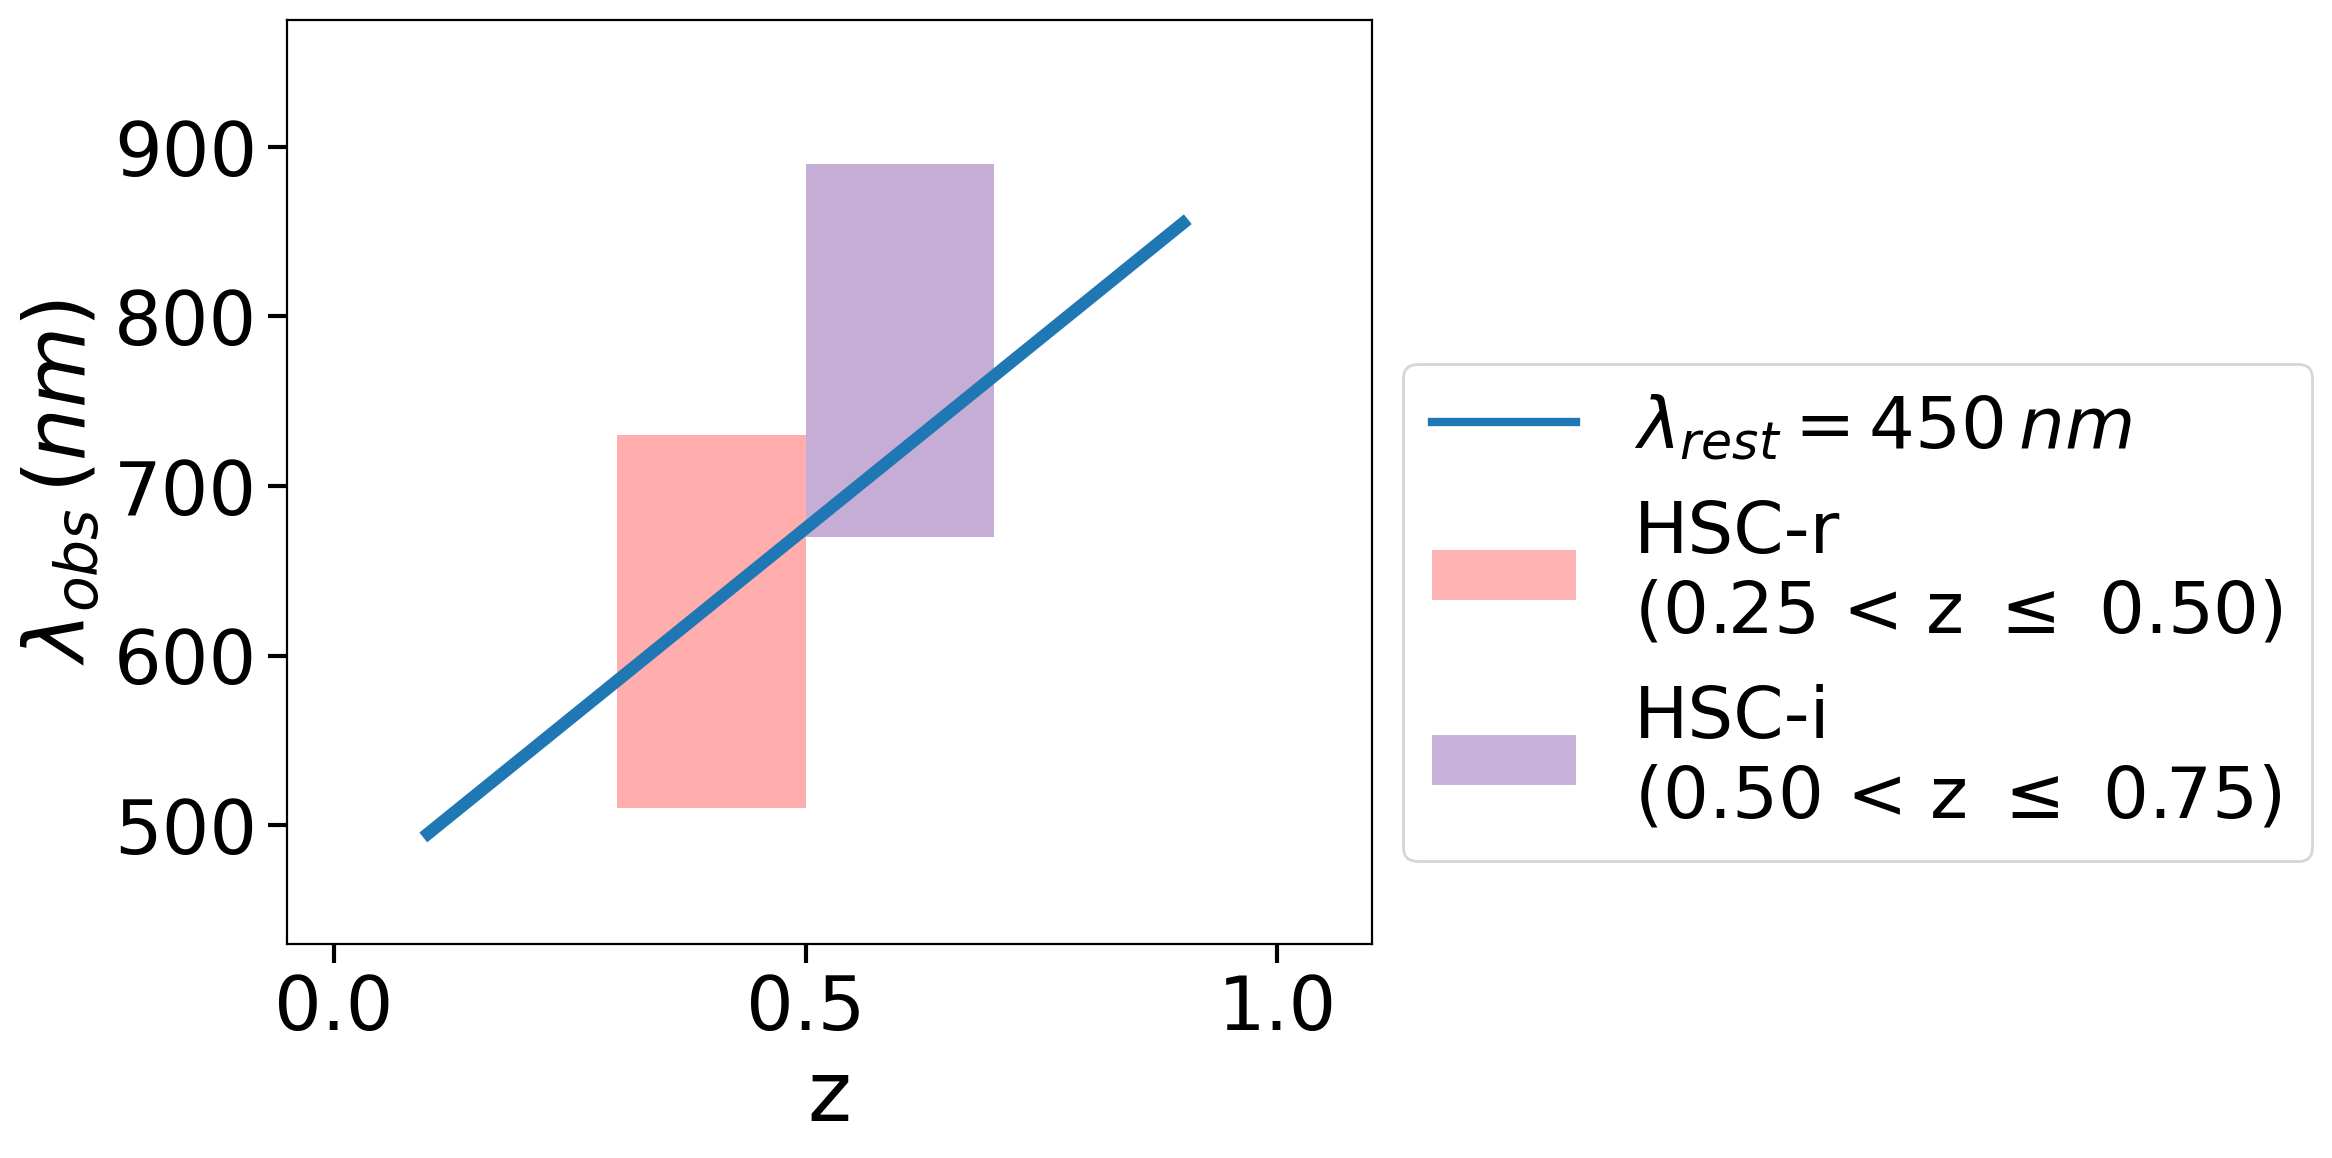
\includegraphics[width = 0.6\textwidth]{band_comp.png}
    \caption{The filter used for each redshift bin is shown along with the wavelength range sampled by each filter. The blue line shows where rest-frame $450$ nm emission falls for redshifts labeled on the x-axis. As this figure shows, the chosen filters allow us to consistently perform morphology determination in the rest-frame \gb{}-band.}
    \label{fig_c4:band_comp}
\end{figure}

As shown in Figure \ref{fig_c4:band_comp}, we consistently perform morphology determination in the rest-frame \gb-band across our entire sample by using  different filters for galaxies at different redshifts. We use \rb-band for $0.3 \leq z < 0.50$, and \ib-band for $0.50 \leq z < 0.7$. We also investigated the effect of color gradients on our measured $R_e$ values by correcting them to a rest-frame wavelength $450nm$. We found the applied size corrections to be pretty mild and $<5\%$ for $0.3 \leq z < 0.5$ galaxies and $<10\%$ for $0.5 \leq 0.7$ galaxies. Additionally, the size corrections had no measurable impact on the primary takeaways of this study. 

For all structural parameters used in this study, we use the most probable value (mode) of the \gampen{}-predicted posterior distributions as the measured value and the width of the $68\%$ confidence interval as the error bar. Note that all measurements used in this study, as well as the ML models used to obtain them, are publicly available \citep{hsc_wide_morphs}.

\subsection{Density Measurements} \label{sec_c4:density_measurements}

\begin{figure*}[htb]
    \centering
    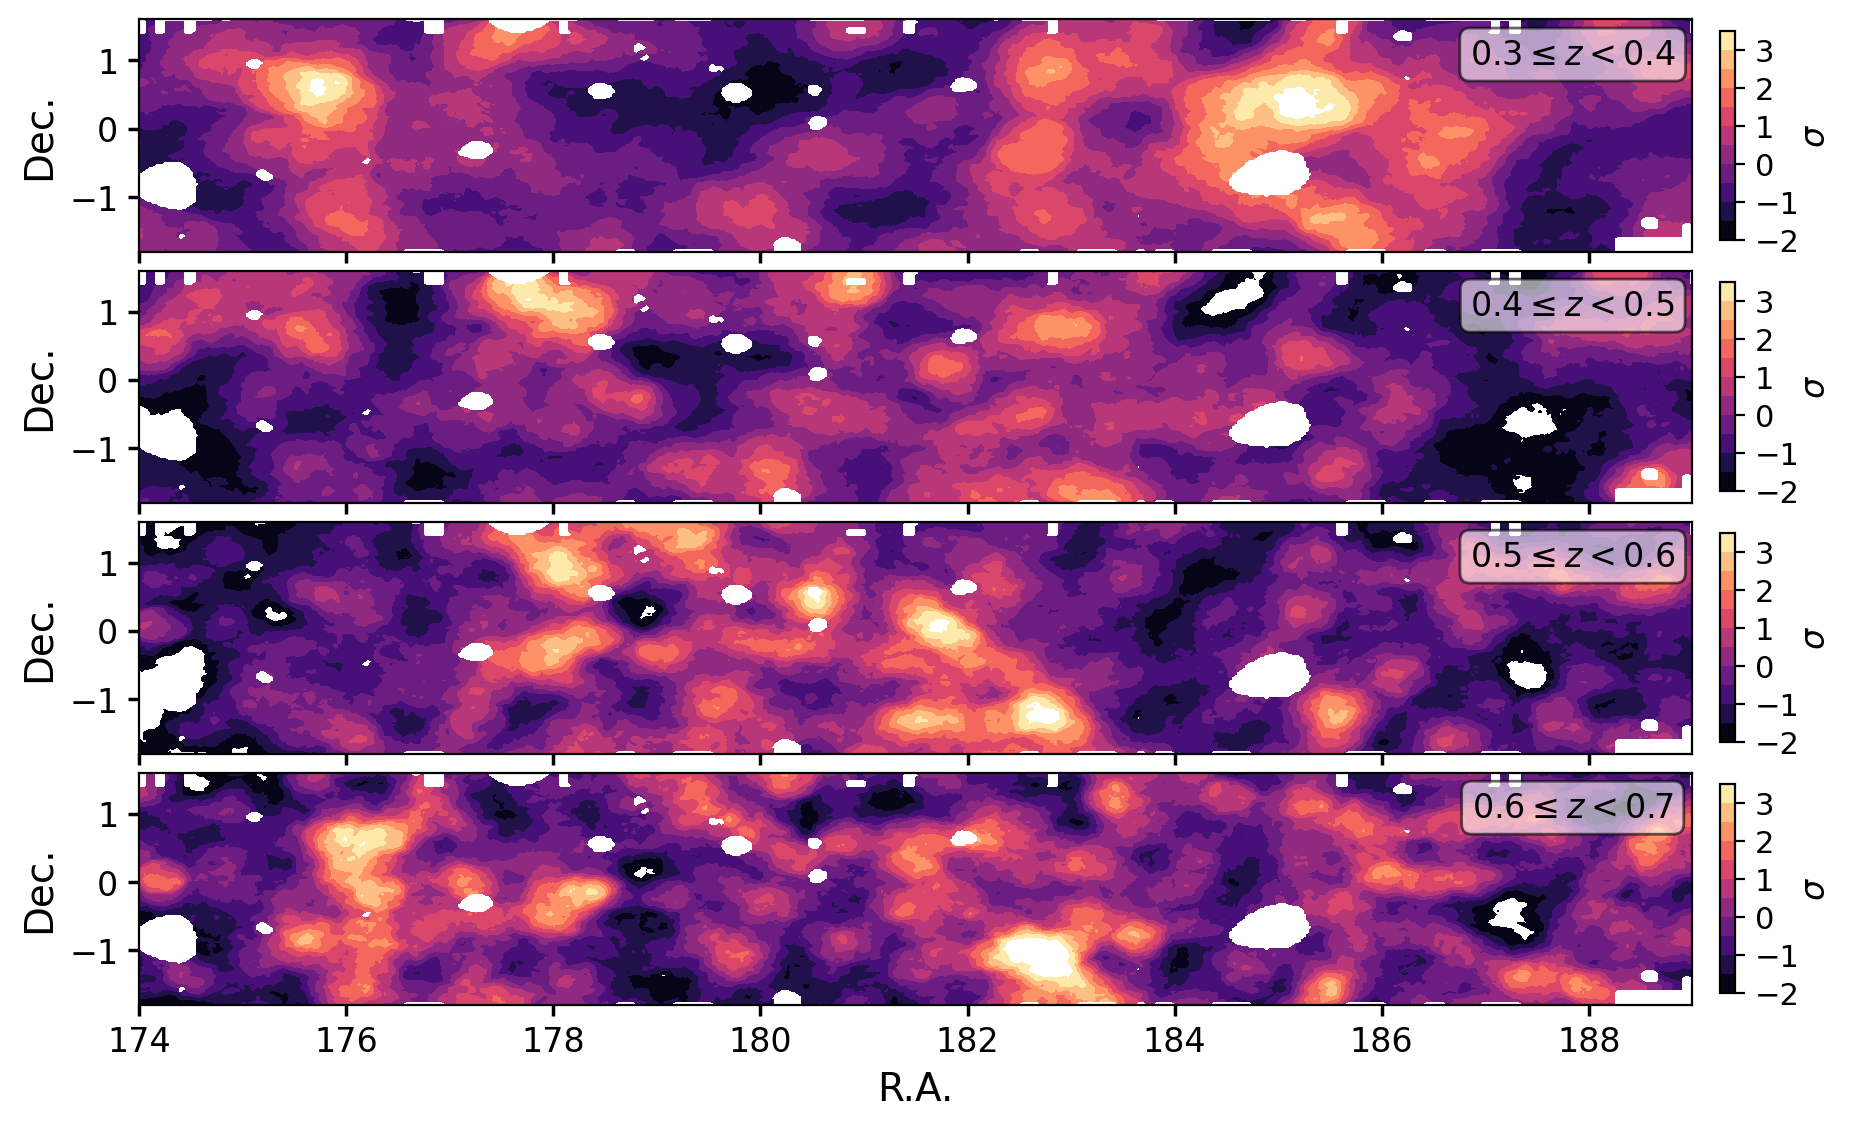
\includegraphics[width = \textwidth]{hsc_den_map.png}
    \caption{Projected two-dimensional densities for one of the HSC-Wide fields at the different redshift slices covered by this study. Colors indicate the density excess in standard deviation within $r=10$ cMPc as denoted in the color bars. (Add scale of 10cMPc at each redshift for comparison)}
    \label{fig_c4:hsc_den_map}
\end{figure*}

The density measurements used in this study are taken from \citet{hsc_den}, which measured the projected two-dimensional density in five of the seven HSC-Wide fields, covering an area of $\sim 360$ deg$^2$. One of the five fields (\texttt{W04 GAMA12H}) is shown as an example in Figure \ref{fig_c4:hsc_den_map}. \citet{hsc_den} chose the $\sim 360$ deg$^2$ survey area by identifying regions in which five sigma limiting magnitude of the point-spread function is deeper than $i=26$ -- this criterion was chosen to prevent the need for correction of the variance of number densities due to depth variation across the survey field. Note that both this study and \citet{hsc_den} use the same underlying based catalog (HSC PDR2) and thus all used measurements (e.g., photometric redshifts) are totally consistent among the studies. 

The projected density map has a spatial resolution of $\sim1.5\arcmin$ and the redshift slices constructed in this study mirror the ones used in \citet{hsc_den}. We set our density estimate at each grid point to be the value of density excess measured using a top-hat aperture of $r=10$ co-Mpc ($\sigma_{r=10 cMpc}$) within the specific redshift slice. Note that \citet{hsc_den} tested their pipeline on a mock galaxy catalog and found that their projected over-densities well trace the total masses of embedded massive dark matter halos at each redshift slice. They also confirmed the consistency of their measurements at $z \leq 0.6$ against mean lens shear signals from a weak lensing stacking analysis. We refer the interested reader to \citet{hsc_den} for more details. 

\subsection{Stellar Masses} \label{sec_c4:mass_completeness}
The stellar masses used in this study come from the same Mizuki catalog that was used for photometric redshift estimates. We remind the reader that our study only includes sources with more than five sigma detection in all HSC bands and we have also discarded sources with reduced chi-square $\chi_{\nu}^2 > 5$ for the best-fitting model. \citet{hsc_photoz_pdr1} and \citet{hsc_morph_den} have compared these stellar masses from Mizuki, based on HSC \gb{}\rb\ib\zb\yb photometry, against stellar masses obtained from the NEWFIRM Medium Band Survey \citep{newfirm} and COSMOS2015 \citep{cosmos_2015}; both of which are based on $>30$-band photometry. Both the above studies found the Mizuki measurements to be overestimates, especially at higher redshifts. However, at $z \leq 0.7$, this discrepancy is $\lesssim0.1$ dex. Note that these differences can be attributed to the systematic differences in the data as well as the adopted templated error functions and priors. Note that when comparing two independent surveys, stellar mass offsets of $\sim0.2-0.3$ dex can be expected even when both the data sets have deep photometry in multiple filters \citep{dokkum_14}.

\begin{figure}[htb]
    \centering
    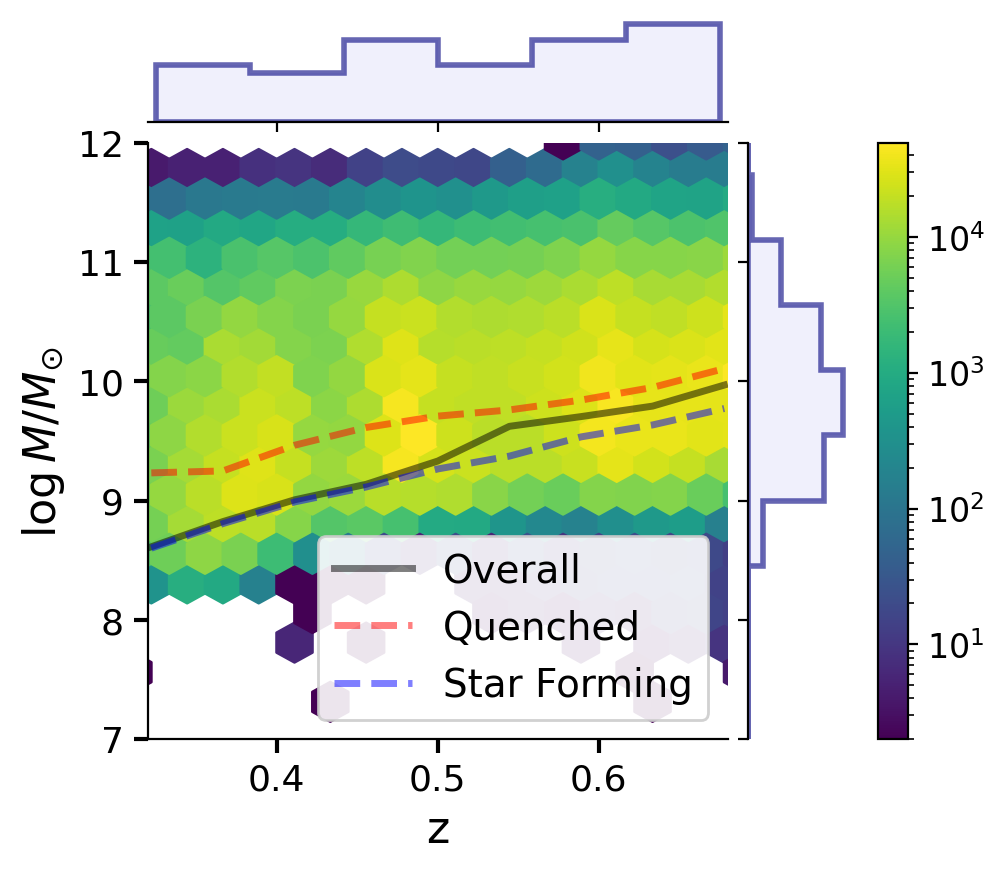
\includegraphics[width = 0.6\textwidth]{mass_comp_marg.png}
    \caption{Distribution of stellar masses as a function of redshift for all galaxies in our sample. The figure shows galaxies in hexagonal bins of roughly equal size, with the number of galaxies in each bin represented according to the colorbar on the right. Marginal histograms are also plotted along each axis. The solid black line shows the $90\%$ stellar mass completeness limit for the entire sample of galaxies. the red and blue dotted lines show the stellar mass completeness limits for the quiescent and star-forming galaxies respectively.}
    \label{fig_c4:mass_comp}
\end{figure}

To estimate the $90\%$ stellar completeness limit of our sample, we follow the approach outlined in \citet{pozzetti_10, Weigel16}. We select galaxies in narrow redshift bins and calculate their limiting stellar mass ($M_{lim}$) -- the mass they would have if their apparent magnitude was equal to $23$, the magnitude limit we chose for our sample. Thereafter, we selected $20\%$ of the faintest galaxies -- and defined the stellar mass completeness limit as the $90^{th}$ quantile  of $M_{lim}$ values in each redshift bin. Figure \ref{fig_c4:mass_comp} shows the determined mass completeness limit for all galaxies; as well as separate completeness limits for star-forming and quiescent galaxies (refer to \S \ref{sec_c4:sep_into_subsamples} for a description of how we classify the sub-samples). Our sample is complete down to $\sim8.5 M_{\odot}$ at $z=0.3$ and $\sim10M_{\odot}$ at $z=0.7$. The completeness limit at the lowest and highest redshifts are 8.6$M_{\odot}$ (9.2$M_\odot$) and 9.9$M_\odot$ ($10.1 M_\odot$) for star-forming (quiescent) galaxies respectively. 

\subsection{Separating Into Sub-Poulations} \label{sec_c4:sep_into_subsamples}
In \S \ref{sec_c4:results}, we will explore the variations of structural parameters v/s environmental density for various sub-populations of galaxy derived from our main sample. To divide galaxies into disk- and bulge-dominated samples; we classify all galaxies with $L_B/L_T \leq 0.4$ as disk-dominated and all galaxies with $L_B/L_T \geq 0.6$ as bulge-dominated. 

To separate galaxies into star-forming and quiescent sub-samples we use their rest-frame SDSS \uband{}-\rb{} v/s \rb{}-\zb{} color-color diagram, which has been shown to be an effective way to separate these sub-populations \citep[e.g.,][]{Holden12, Chang15, lopes_16, hsc_mass_size}. Note that for our sample, we are unable to use \textit{UVJ} selection because SED fitting using HSC \grizy{} photometry does not allow us to obtain robust estimates for rest-frame {J} magnitudes. We obtain the SDSS rest-frame magnitudes from the same Mizuki catalog that was used for redshift and stellar mass estimation. 

\citet{hsc_mass_size} has demonstrated that applying the \citet{Holden12} \textit{urz} color selection directly to HSC data does not optimally distinguish the quiescent and star-forming galaxies; instead, the boundaries need to be adjusted. Thus, we follow \citet{Kawin16} and \citet{hsc_mass_size}, and use our sample to self-calibrate the region separating quiescent from star-forming galaxies. The final separation boundaries obtained, along with an extended description of the procedure, are available in Appendix \ref{sec_c4:ap:cc_sel}.

\section{Results} \label{sec_c4:results}
The central focus of this work is to study how the structural parameters of galaxies (with similar masses) vary as a function of their environmental density. In \S \ref{sec_c4:data}, we already described how a measurement of environmental density is assigned to (a sample of) galaxies from the \citet{hsc_wide_morphs} morphological catalog. We now use this combined information to study how environment affects galaxy radius (\S \ref{sec_c4:rad_den}); and how the measured fractions of different morphological classes change as a function of environment (\S \ref{sec_c4:morph_env}).

\subsection{Variation of Radius with Environment} \label{sec_c4:rad_den}
We bin the galaxies in each redshift slice into five bins based on their environmental density. The bins are linearly spaced and span the range $\sigma_{r=10cMPc} = [-2,3]$. Thereafter, within each bin, we investigate the distribution of half-light radius ($R_e$). In \S \ref{sec_c4:rad_den_all}, we will outline our results for all galaxies in our sample; and in \S \ref{sec_c4:rad_den_sub}, we will focus on four specific subpopulations of galaxies -- disk-dominated, bulge-dominated, star-forming, and quiescent. 

\subsubsection{All Galaxies} \label{sec_c4:rad_den_all}
\begin{figure*}[htb]
    \centering
    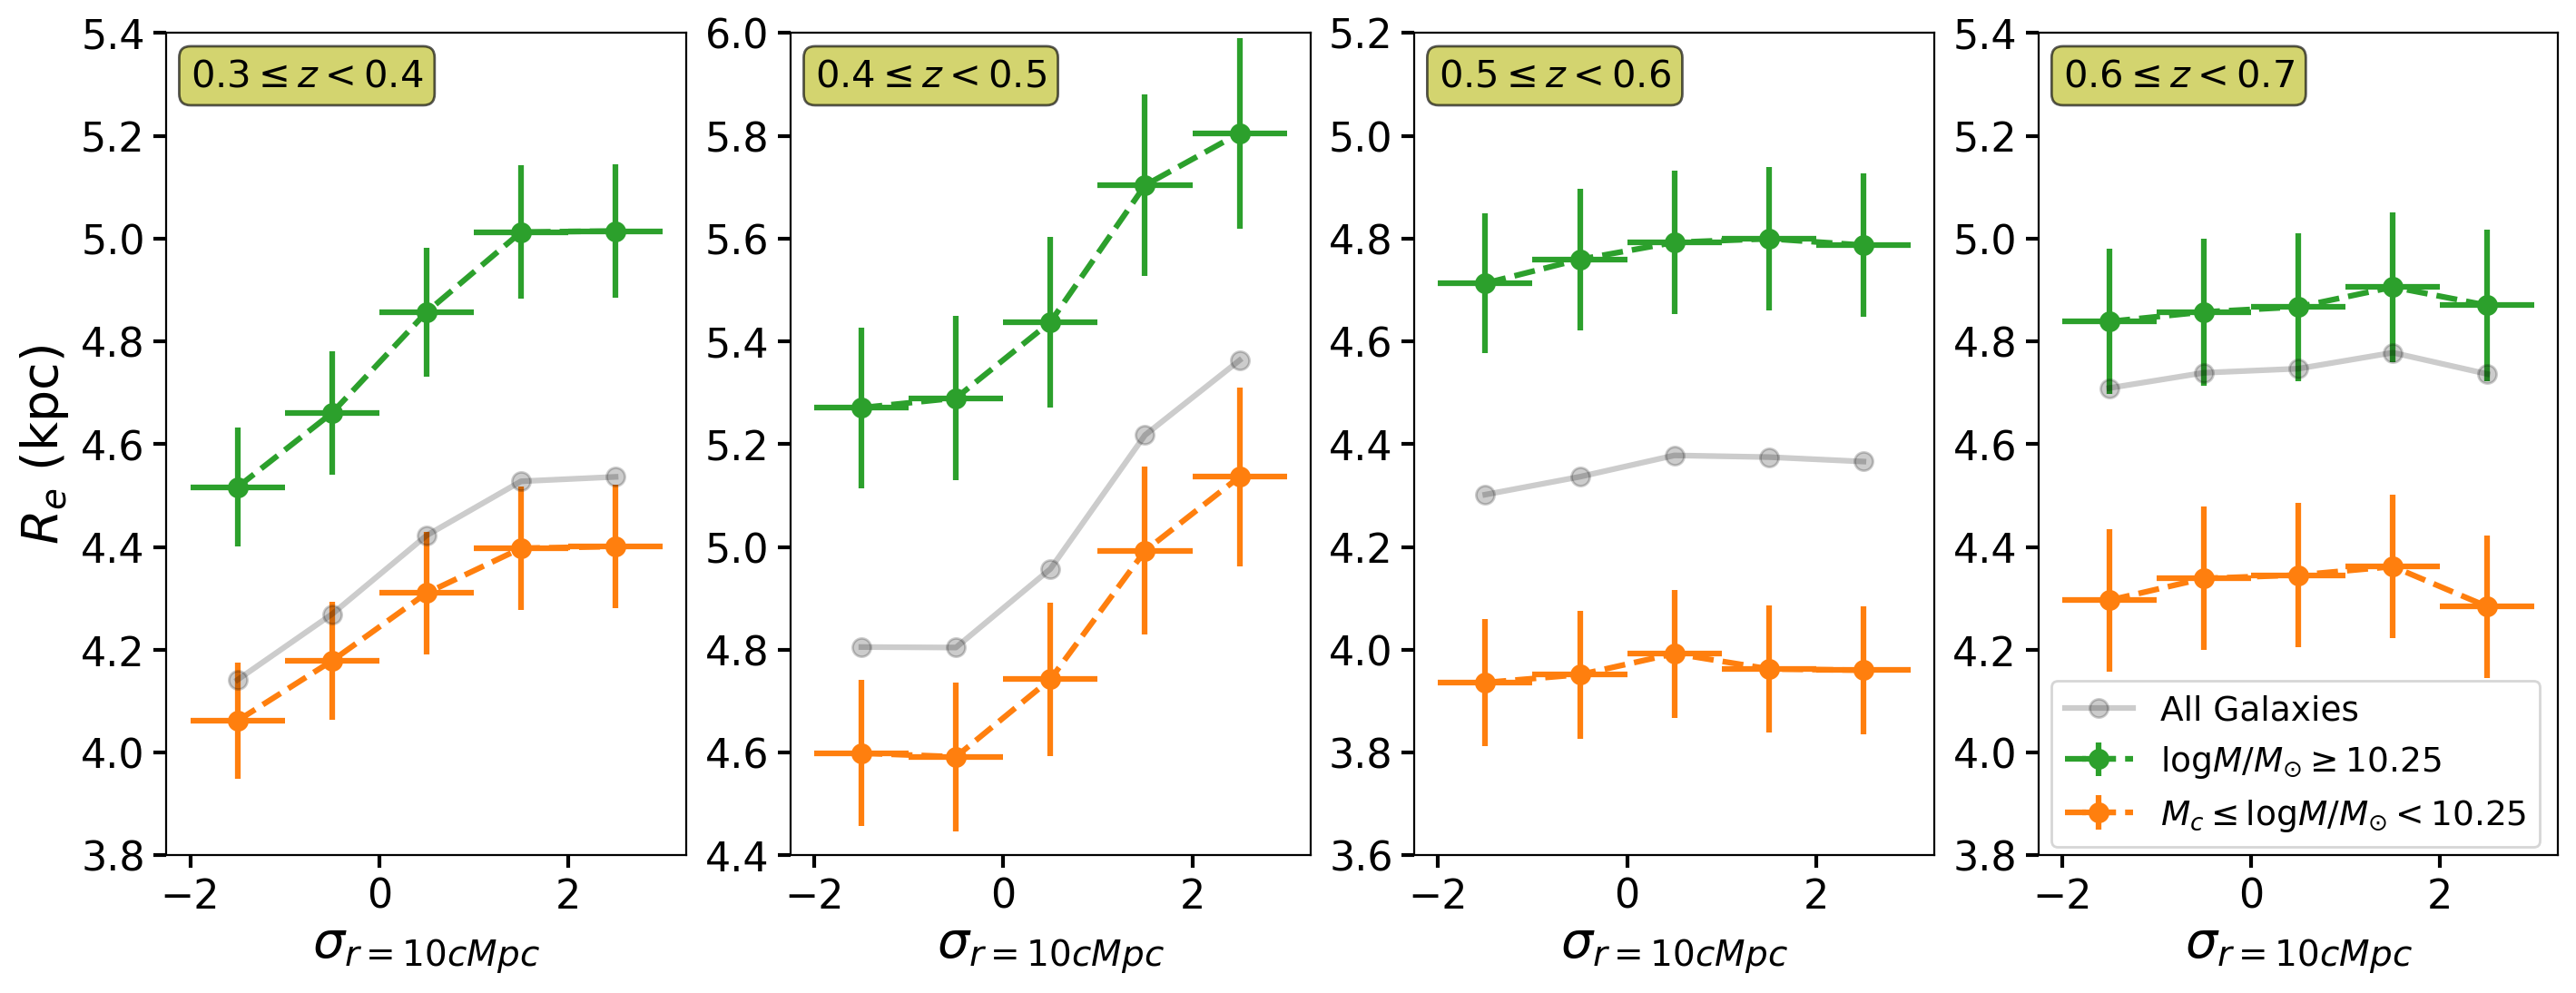
\includegraphics[width = \textwidth]{rad_den_all.png}
    \caption{Effective radius v/s density excess at different redshifts (different panels) shown in limited ranges of stellar mass (different colored lines). The points show the median radius in each bin and the error bars depict the median $68\%$ confidence interval predicted by \gampen{} for all galaxies in that bin. The grey line shows the median trend for the entire sample in the given redshift bin.}
    \label{fig_c4:rad_den_all}
\end{figure*}


\begin{table}
    \centering
    \caption{Statistical Significance of Radius v/s Density Correlations \label{tab_c4:corr_all}}
    \begin{tabular}{c|c|KKKK}
    \hline
    \hline 
    Mass Range & & $0.3 \leq z < 0.4$ & $0.4 \leq z < 0.5$ & $0.5 \leq z < 0.6$ & $0.6 \leq z < 0.7$ \\ 
    ($\log M/M_{\odot}$) & & & & \\
    \hline
    \hline
    \multirow[c]{3}{*}{$\geq10.25$} & $\rho$   & $1.1\times10^{-1} \pm 5.8\times10^{-4}$ & $9.4\times10^{-2} \pm 5.5\times10^{-4}$ & $1.9\times10^{-2} \pm 4\times10^{-4}$ & $1.4\times10^{-2} \pm 4\times10^{-4}$ \\
                                    & $p$      & $4.7\times10^{-210} \pm (<10^{-300})$ & $4.9\times10^{-193} \pm (<10^{-300})$ & $3.9\times10^{-9} \pm 4.6\times10^{-9}$ &  $1.8\times10^{-5} \pm 1.3\times10^{-5}$   \\
                                    & $\alpha$ & $185\sigma_{\rho}$ & $169\sigma_{\rho}$ & $46\sigma_{\rho}$ & $33\sigma_{\rho}$  \\
                                    & $>5\sigma$ & \checkmark & \checkmark &  \checkmark &   \\
    \hline
    \multirow{3}{*}{$\left[9.5,10.25\right)$} & $\rho$ & $5.7\times10^{-2} \pm 4.7\times10^{-4}$   & $1\times10^{-1} \pm 5.9\times10^{-4}$ & $1.6\times10^{-2} \pm 4.5\times10^{-4}$ & $9.1\times10^{-3} \pm 5.2\times10^{-4}$ \\
                                                & $p$  & $4.8\times10^{-73} \pm 7.6\times10^{-71}$ & $1.8\times10^{-219} \pm (<10^{-300})$ & $4.8\times10^{-7} \pm 5.4\times10^{-7}$ &  $3.9\times10^{-3} \pm 2.3\times10^{-3}$   \\
                                             & $\alpha$ & $122\sigma_{\rho}$ & $170\sigma_{\rho}$ & $35\sigma_{\rho}$ & $17\sigma_{\rho}$  \\
                                             & $>5\sigma$ & \checkmark & \checkmark &  &   \\
    \hline
    \multirow{3}{*}{$<9.5$} & $\rho$ & $9.5\times10^{-2} \pm 5.9\times10^{-4}$   & $9.7\times10^{-2} \pm 7.4\times10^{-4}$ & $2.9\times10^{-2} \pm 5.7\times10^{-4}$ & $4.4\times10^{-3} \pm 6.1\times10^{-4}$ \\
                            & $p$  & $2.9\times10^{-199} \pm (<10^{-300})$ & $3.4\times10^{-209} \pm (<10^{-300})$ & $2.2\times10^{-20} \pm 2.4\times10^{-19}$ &  $1.7\times10^{-1} \pm 6.2\times10^{-2}$   \\
                            & $\alpha$ & $160\sigma_{\rho}$ & $132\sigma_{\rho}$ & $51\sigma_{\rho}$ & $7\sigma_{\rho}$  \\
                            & $>5\sigma$ & \checkmark & \checkmark & \checkmark &   \\
    \hline
    \hline
    \multicolumn{6}{p{0.95\textwidth}}{\vskip 0.01cm \small $\rho$ refers to the Spearman correlation coefficient. Median $\pm$ standard deviation values are reported above.} \\
    \multicolumn{6}{p{0.95\textwidth}}{\small $p$ refers to the probability of a spurious correlation. Median $\pm$ standard deviation values are reported above. } \\
    \multicolumn{6}{p{0.95\textwidth}}{\small $\alpha$ refers to the distance between the median value of $\rho$ and $\rho=0$ (signifying no correlation). Reported above in terms of standard deviation (of $\rho$) } \\
    \multicolumn{6}{p{0.95\textwidth}}{\small \checkmark indicates that we can confirm a positive correlation with $\geq 5\sigma$ confidence} \\
    \end{tabular}
\end{table}

Figure \ref{fig_c4:rad_den_all} shows the median value of the effective radius in each density bin. We also split the sample into three mass bins:- $\log M/M_{\odot} < 9.5$, $9.5 \leq \log M/M_{\odot} < 10.5$, and $\log M/M_{\odot} \geq 10.5$. These bins were chosen as $\sim9.5M_{\odot}$ and $\sim10.25M_{\odot}$ correspond to the $25^{th}$ and $75^{th}$ quantiles, respectively, of the stellar mass distribution. The vertical error bar on each point reflects the median $1\sigma$ width of the $R_e$ posterior distribution predicted by \gampen{} for all galaxies in that bin. The four panels show the four different redshift slices, and each color delineates a separate mass range. 

Although Figure \ref{fig_c4:rad_den_all} is an accurate representation of the available data --- it does not fully capture all the information available to us. \gampen{} predicts the full posterior distribution of structural parameters, and thus, for every galaxy in our sample, we have a predicted probability distribution of $R_e$ values. Therefore, judging the existence of correlations by visual inspection alone is not statistically robust in this scenario. Rather, we use a Monte-Carlo sampling technique to incorporate each of these predicted distributions into judging whether a correlation exists or not; and estimate with what statistical significance we can reject the null hypothesis of no-correlation. 

For every galaxy in our sample, we use the predicted posterior distribution to draw 5000 samples of $R_e$, effectively creating 5000 stochastic copies of our dataset. Now for each of these datasets, we use the Spearman's rank correlation test \citep{spearman_original} to judge the existence of a correlation between $R_e$ and $\sigma_{r=10cMPc}$. The Spearman's test is a non-parameteric method to asses how well the relationship between two variables can be described using a monotonic function. The test estimates two variables $\rho$ and $p$. $\rho$ is the correlation co-efficient can takes values between $-1$ to $+1$ with the end limits signifying the variables being perfect monotonic functions of each other. $\rho=0$ signifies no correlation between the variables. The value of $p$ roughly indicates the probability of an uncorrelated system producing datasets that have a Spearman correlation at least as extreme as the computed $\rho$. The above Monte-Carlo procedure results in a distribution of $\rho$ and $p$ values for each mass-bin within the four redshift slices. %We refer an interested reader to Appendix \ref{sec_c4:ap:corr_coeff} for an extended description of the Monte-Carlo procedure and the Spearman test. 

The values of the $p$ and $\rho$ obtained using the procedure above is reported in Table \ref{tab_c4:corr_all}. Note that Table \ref{tab_c4:corr_all} also reports the value of $\alpha$. We define $\alpha$ as the distance between the median value of $\rho$ and $\rho=0$ -- we report it in terms of the standard deviation ($\sigma_{\rho}$) of the $\rho$ distribution. Larger values of $\alpha$ signify stronger and more statistically significant correlation. For p-values, we also report the median and standard deviation of the distribution. The \checkmark{s} in Table \ref{tab_c4:corr_all} signify whether we can reject the null hypothesis of non-correlation at a significance level of 5 sigma or more. To assign a \checkmark, we check whether ($(\overline{p} + \sigma_p) < 3\times10^{-7} $) \texttt{AND} ($\alpha>5\sigma_{\rho}$). 

As can be seen from Table \ref{tab_c4:corr_all} and Figure \ref{fig_c4:rad_den_all}, $0.3 \leq z < 0.5$, we can confirm the existence of a strong positive correlation between $R_e$ and environmental density across the entire mass range probed by this study ---  we find that galaxies in denser environments are consistently larger than galaxies of similar mass in less dense environments. As we move to higher redshifts, the relationship significantly flattens out, with no statistically significant correlation observed for the highest redshift slice. For the $0.5 \leq z < 0.6$, the observed correlations are much weaker, and the for the mid-mass bin, we can only confirm the existence of a correlation at a statistical significance of $>4\sigma$. Note that throughout our sample, the highest mass bin always seems to display a marginally stronger correlation than the lower mass bins. 

\begin{figure*}[htb]
    \centering
    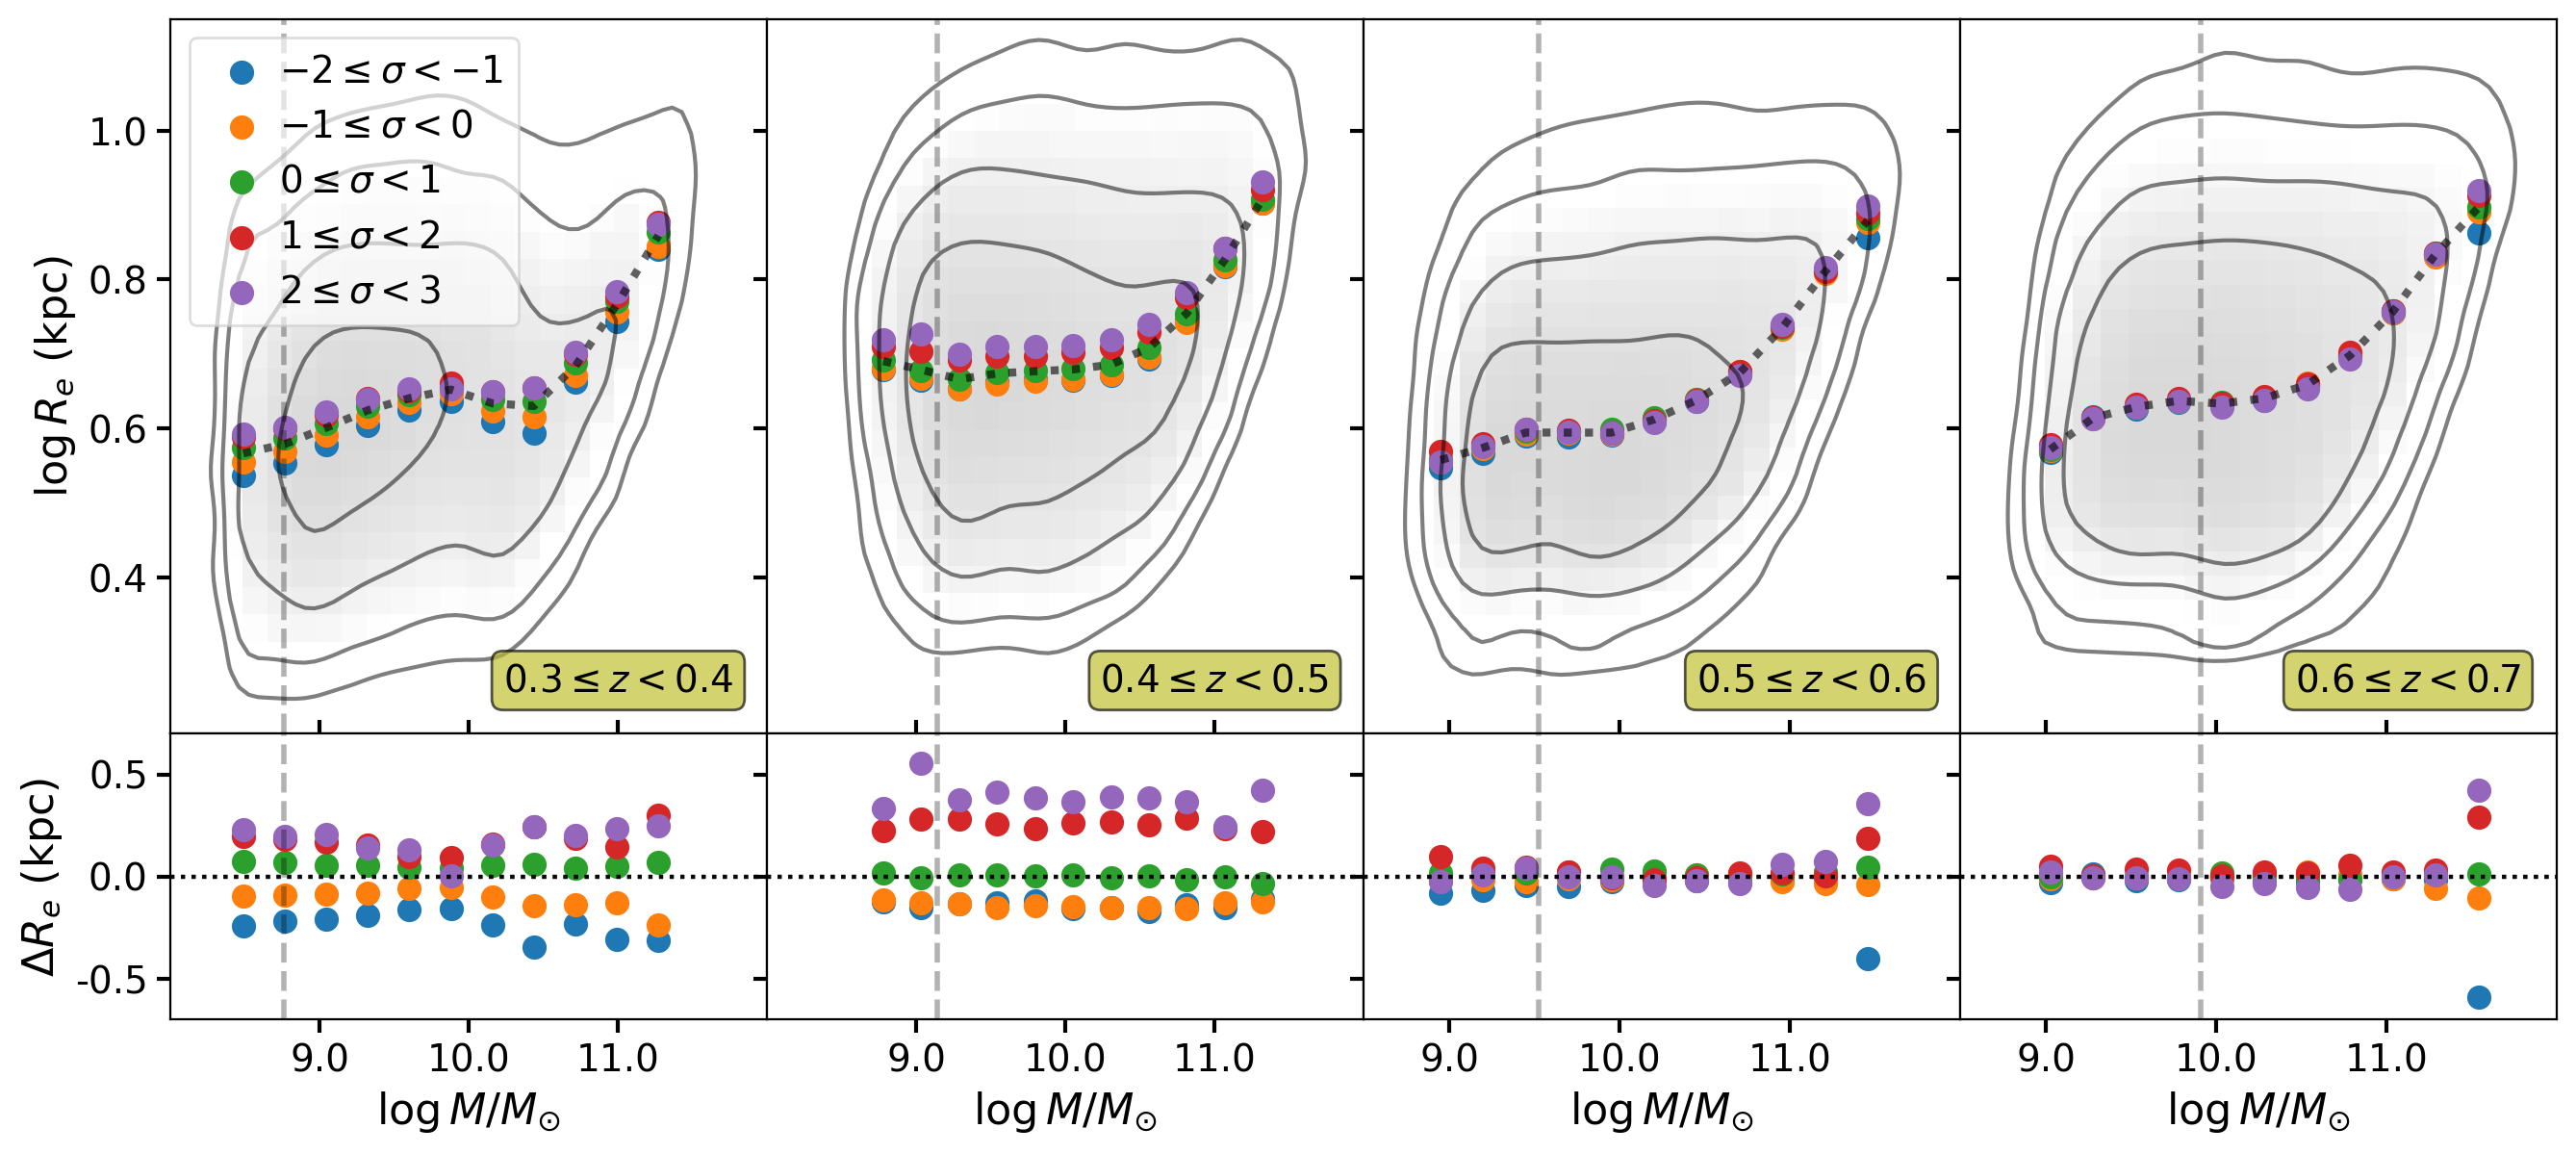
\includegraphics[width = \textwidth]{r_m_all.png}
    \caption{The size-mass relationship shown for the four different redshift slices. The black dotted lines in the upper panels show the median trend; while the colored points show the measurements separately for sub-samples of galaxies in different environments. The grey dotted vertical line running throughout each panel shows the overall mass completeness at each redshift bin. The bottom panel displays how the colored points deviate from the overall median trend.}
    \label{fig_c4:r_m_all}
\end{figure*}

To investigate the $R_e$ v/s $\sigma_{r=10cMPc}$ in finer mass bins, we plot the size-mass relationship for our sample in Figure \ref{fig_c4:r_m_all} and investigate the locations of galaxies in different environments on the size-mass plane. The contour and shading in the top panel delineate denser regions of the size-mass plane; and the black dotted line shows the overall trend. The colored points show the median $\log(R_e)$ of galaxies in different environments within each mass bin. The bottom panels show how the colored points deviate from the median trend line. 

For the lower two redshift bins, Figure \ref{fig_c4:r_m_all} confirms what we saw previously -- we consistently find that galaxies in denser environments are larger (by $\sim 0.5-0.7$ kpc) than galaxies of similar mass in less dense environments. For the two higher z-bins, the overall effect is much weaker/absent, consistent with what we found earlier. However Figure \ref{fig_c4:r_m_all} adds a new dimension to our results in the $z \geq 0.5$ bins -- there appears to be a critical stellar mass, above which we can observe a correlation between radius and environment. The effect is significantly stronger than what can be observed for less massive galaxies at these higher redshifts. In Figure \ref{fig_c4:r_m_all}, although this effect is visible over primarily one mass-bin, we have verified that when we use finer mass bins, we observe a `ramping up' of this effect for $log M/M_{\odot} > 10^{11.25} \sim 2\times10^{11}$. We ran the Monte-Carlo correlation analysis specifically for galaxies above this critical stellar mass and observed the following values:- $\rho = 5.5\times10^{-2} \pm 1.42\times10^{-3}$, $p = 3\times10^{-13} \pm 3.2\times10^{-12}$, $\alpha=32\sigma_{\rho}$ for the $0.5 \leq z < 0.6$ slice; and $\rho = 5\times10^{-2} \pm 1.3\times10^{-3}$, $p = 1.4\times10^{-17} \pm 3.6\times10^{-16}$, $\alpha=36\sigma_{\rho}$. Therefore, we have more than enough statistics at these higher masses to confirm the correlation with $>5\sigma$ confidence. Note that the existence of this high critical stellar mass might explain why some of the studies in Table \ref{tab_c4:lit_survey} didn't observe any correlation; as many of them did not probably have enough statistics at these very high masses. 

In Figure \ref{fig_c4:r_m_all}, we also observe the existence of a mass-dependant slope of the size-mass relationship across all the four redshift bins. The slope of the size-mass relationship is shallower at lower masses, with a pivotal stellar mass above which the slope becomes much steeper. This effect has been observed previously across a wide redshift range and it has been posited that the pivotal stellar mass represents a mass above which both the stellar mass growth and the size growth of galaxies transition from being star formation dominated to dry mergers dominated \citep[e.g.,][]{mowla19,hsc_mass_size}. The observed pivotal stellar masses ($\log M/M_{\odot} \sim 10.3-10.6$) is consistent with what has been observed previously; and we can additionally confirm that the pivotal stellar mass does not appear to be dependant on environmental density. 

\subsubsection{Specific Subsamples} \label{sec_c4:rad_den_sub}

%\begin{figure*}[htb]
%    \centering
%    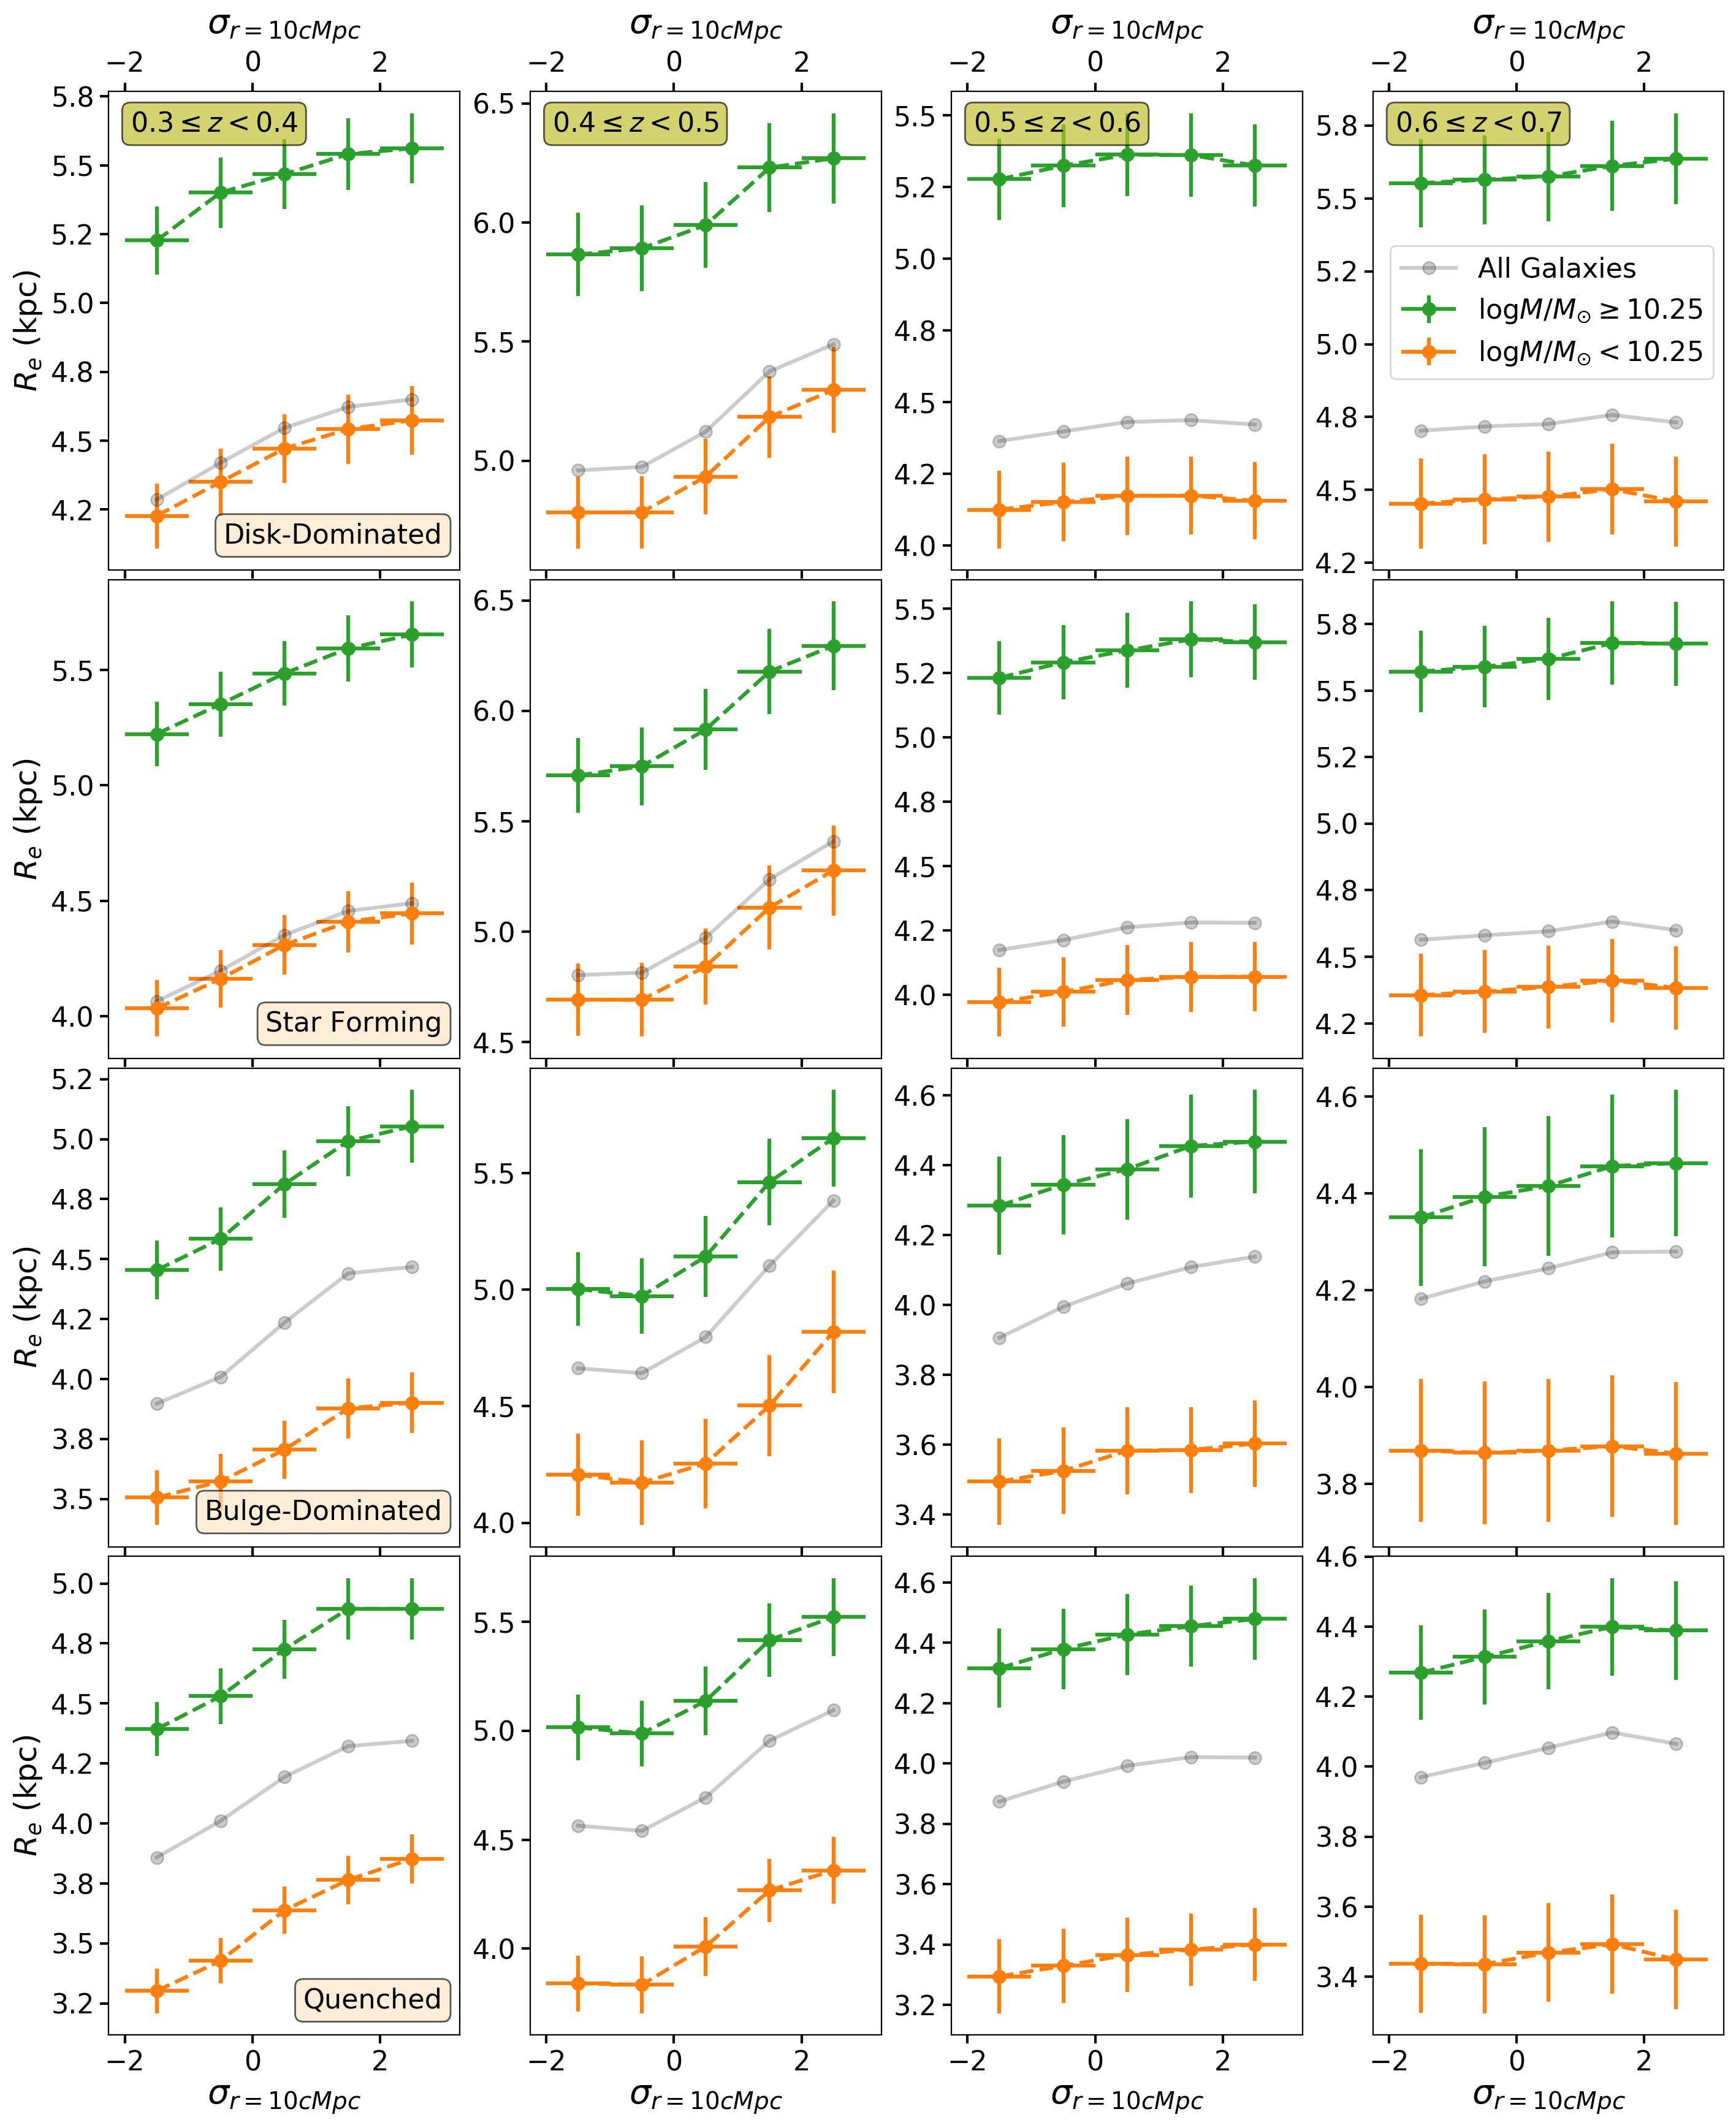
\includegraphics[width = 0.85\textwidth]{rad_den_sub.png}
%    \caption{Effective radius v/s density excess at different redshifts (different columns) shown for different sub-samples of galaxies (different rows). The points show the median radius in each bin and the error bars depict the median $68\%$ confidence interval predicted by \gampen{} for all galaxies in that bin. The grey line shows the median trend for the entire sample in the given redshift bin. Note that we merged the two lower mass bins used in Figure \ref{fig_c4:rad_den_all} into one bin in this Figure to ensure statistically significant sample sizes in each measurement bin.}
%    \label{fig_c4:rad_den_sub}
%\end{figure*}

\begin{figure*}
    \begin{center}
        \subfigure{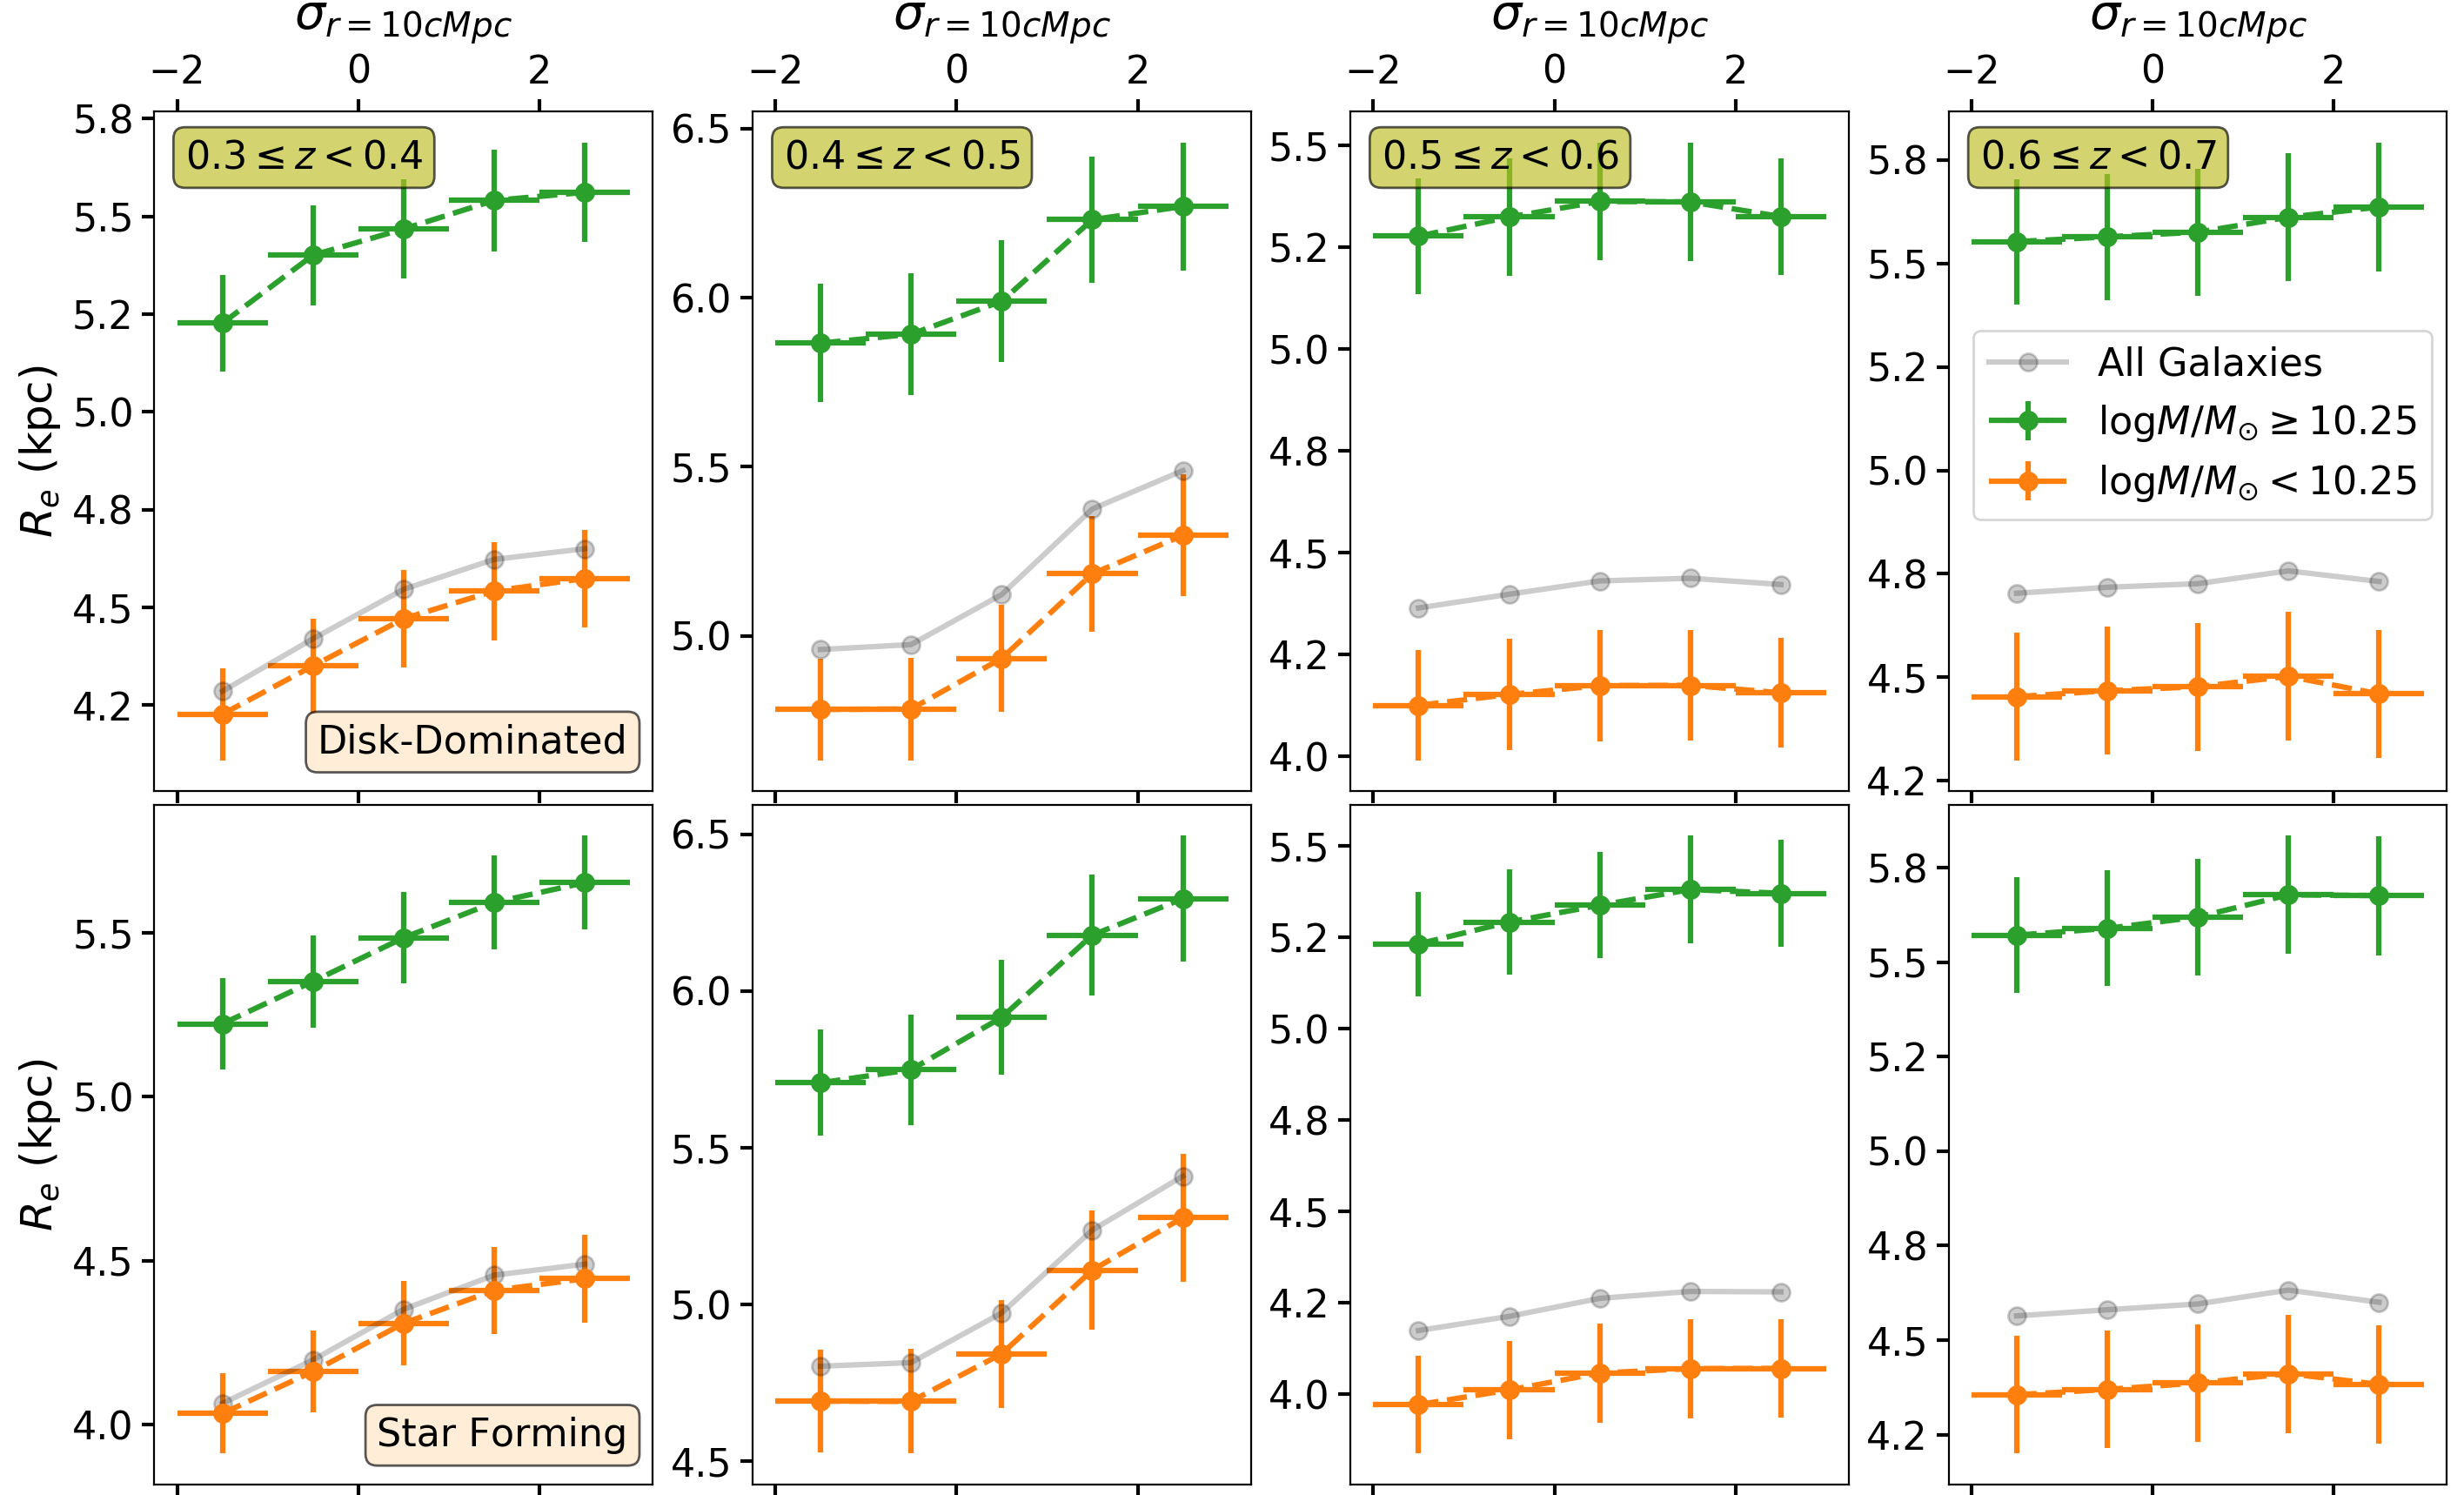
\includegraphics[width=\textwidth]{rad_den_sub_1.png}} 
        \subfigure{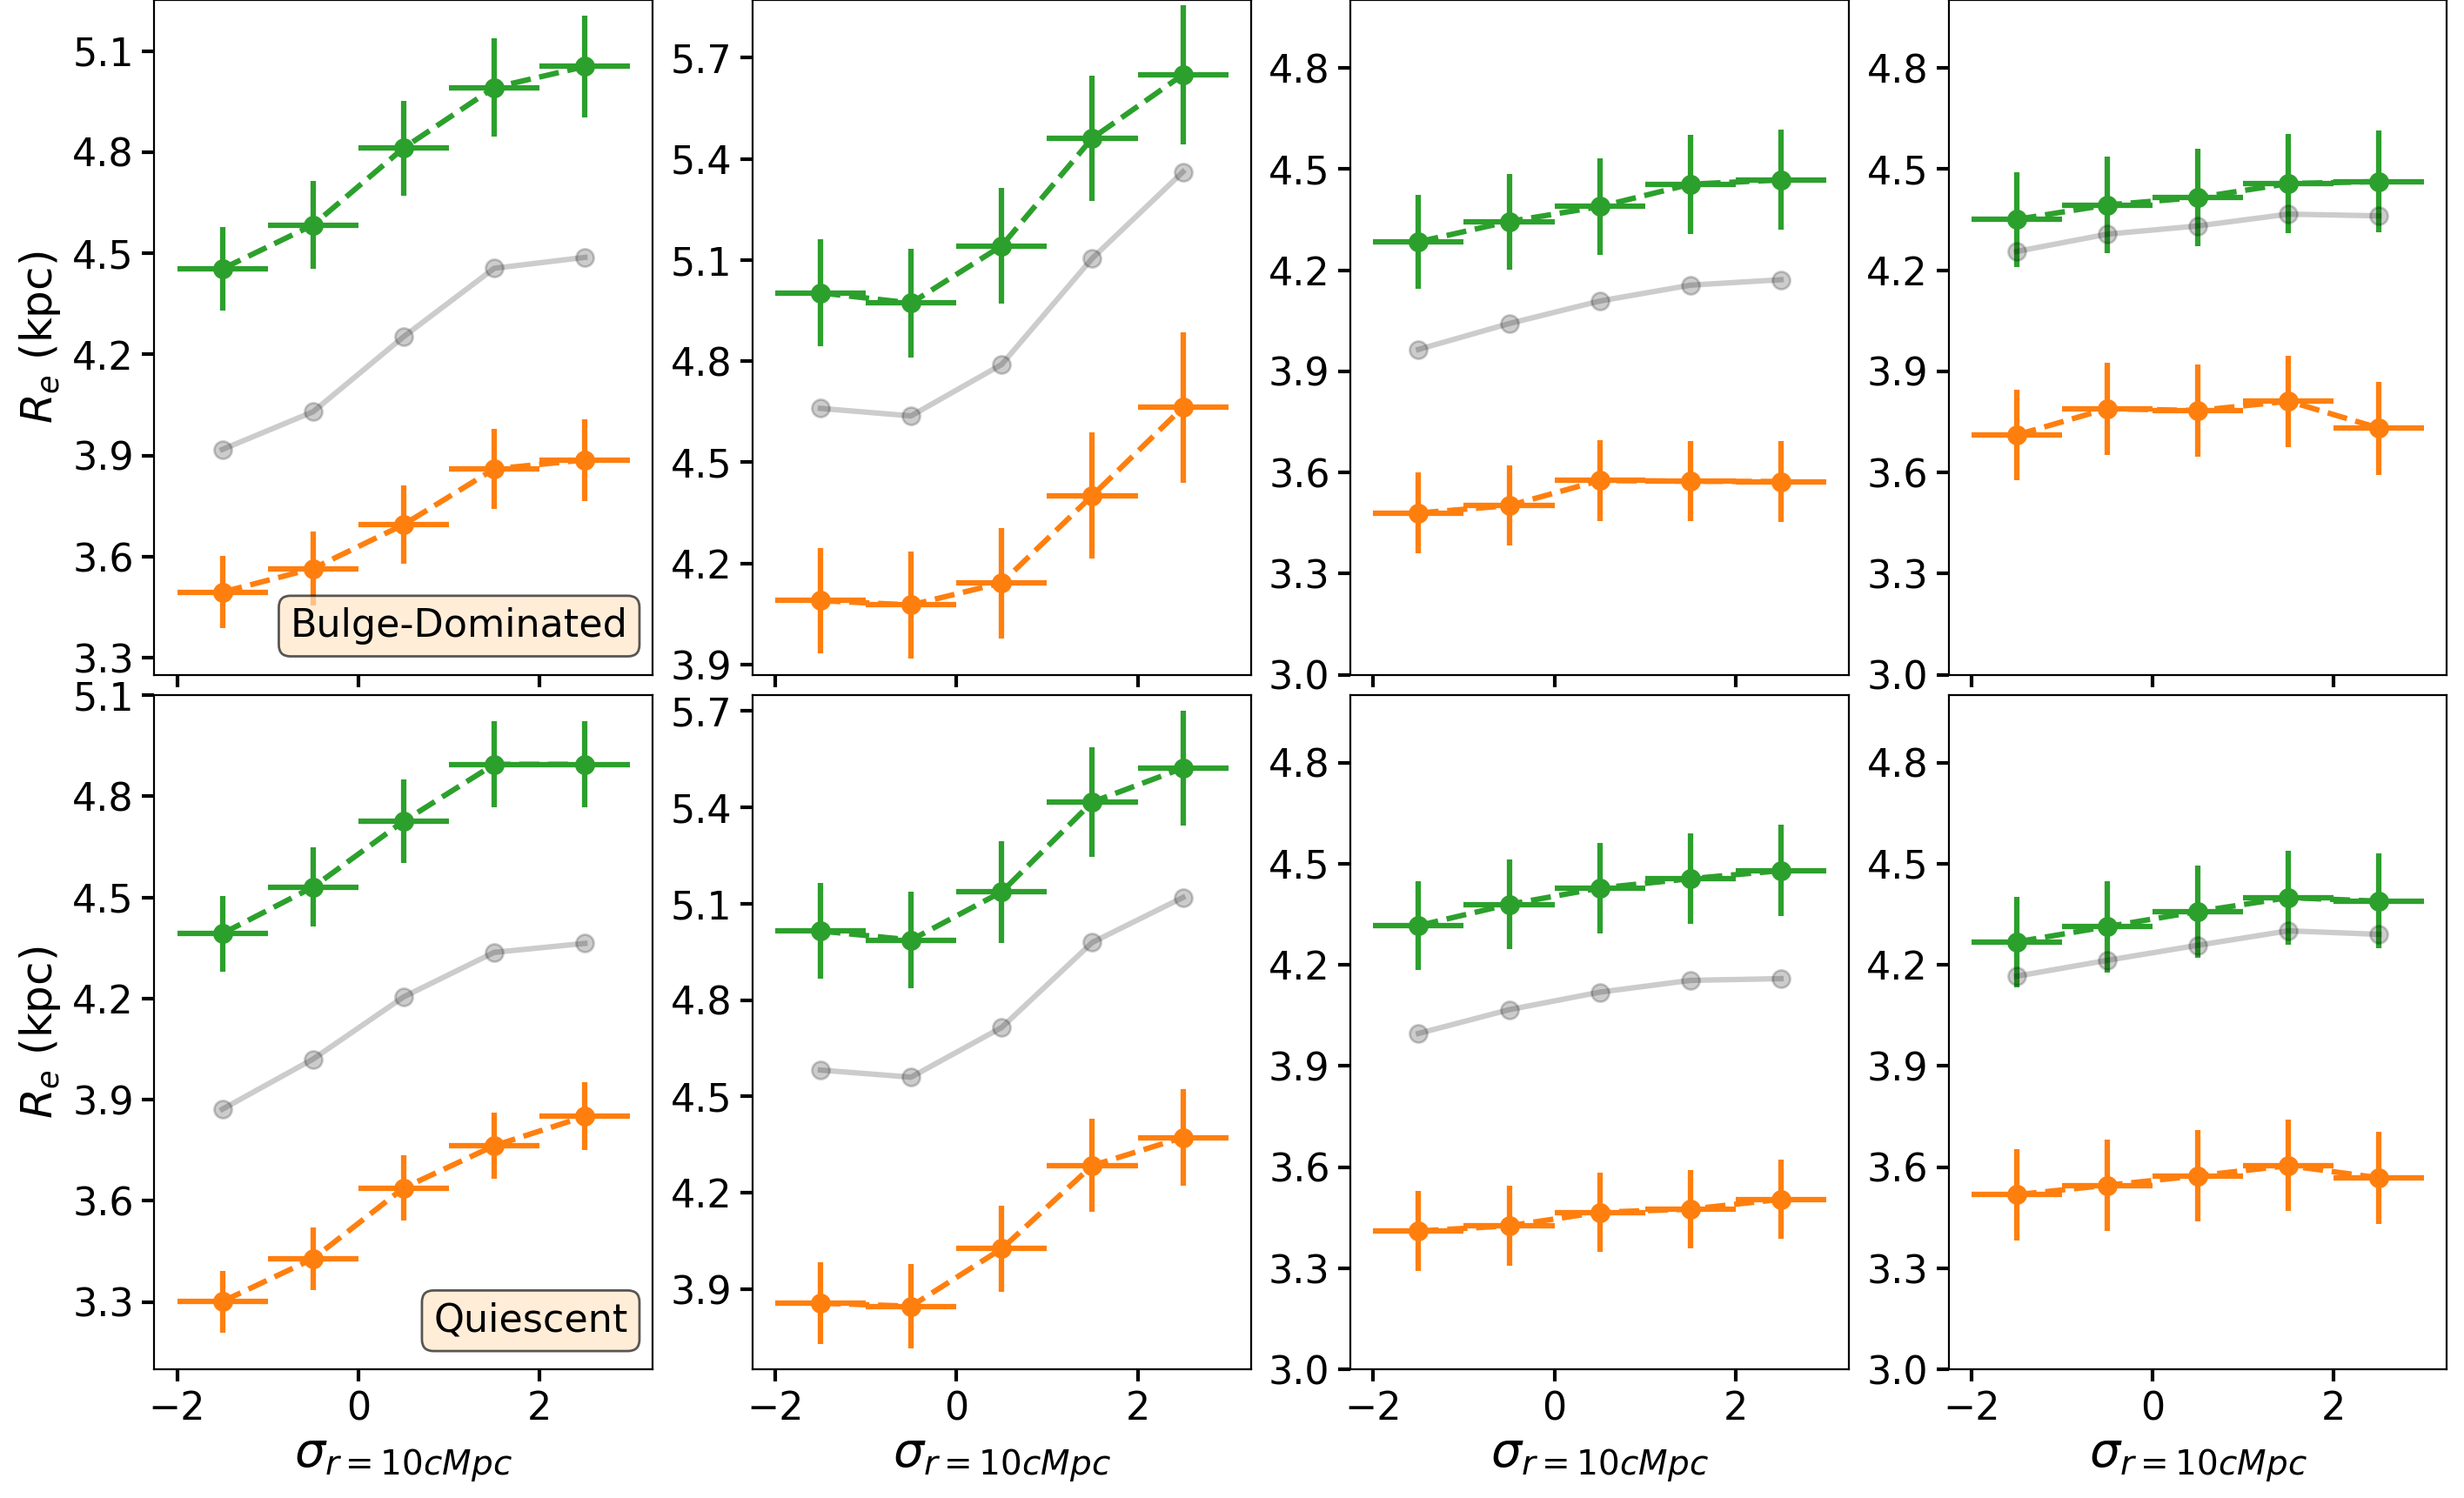
\includegraphics[width=\textwidth]{rad_den_sub_2.png}} 
  \end{center}
  \caption{Effective radius v/s density excess at different redshifts (different columns) shown for different sub-samples of galaxies (different rows). The points show the median radius in each bin and the error bars depict the median $68\%$ confidence interval predicted by \gampen{} for all galaxies in that bin. The grey line shows the median trend for the entire sample in the given redshift bin. Note that we merged the two lower mass bins used in Figure \ref{fig_c4:rad_den_all} into one bin in this Figure to ensure statistically significant sample sizes in each measurement bin.}
    \label{fig_c4:rad_den_sub}
\end{figure*}

\begin{table}
    \centering
    \caption{Statistical Significance of Radius v/s Density Correlations for Galaxy Sub-Populations \label{tab_c4:corr_subpop_ab}}
    \begin{tabular}{>{\centering\arraybackslash}p{2cm}|c|c|cccc}
        \hline
        \hline
        Sub-Population & Mass Range & & $0.3 \leq z < 0.4$ & $0.4 \leq z < 0.5$ & $0.5 \leq z < 0.6$ & $0.6 \leq z < 0.7$ \\ 
          & ($\log M/M_{\odot}$) & & & & \\
        \hline
        \hline 
        \multirow{8}{*}{Disk Dom.} & \multirow[c]{4}{*}{$\geq10.25$} & $\rho$   & $\om(10^{-2})$ & $\om(10^{-2})$ & $\om(10^{-2}$ & $\om(10^{-2})$ \\
                                    &                                  & $p$      & $\om(10^{-13})$ & $\om(10^{-101})$ & $\om(10^{-9})$ &  $\om(10^{-8})$   \\
                                    & & $\alpha$ & $49\sigma_{\rho}$ & $89\sigma_{\rho}$ & $47\sigma_{\rho}$ & $44\sigma_{\rho}$  \\
                                    & & $>5\sigma$ & \checkmark & \checkmark &  Borderline \checkmark &  Borderline \checkmark \\
                 \cline{2-7}
                 & \multirow[c]{4}{*}{$<10.25$} & $\rho$   & $\om(10^{-2})$ & $\om(10^{-1})$ & $\om(10^{-2})$ & $\om(10^{-3})$ \\
                                    &             & $p$      & $\om(10^{-92})$ & $\om(10^{-252})$ & $\om(10^{-7})$ &  $\om(10^{-2})$   \\
                                    & & $\alpha$ & $127\sigma_{\rho}$ & $188\sigma_{\rho}$ & $32\sigma_{\rho}$ & $14\sigma_{\rho}$  \\
                                    & & $>5\sigma$ & \checkmark & \checkmark &  &  \\
    \hline
    \hline
    \multirow{8}{*}{Star-Forming} & \multirow[c]{4}{*}{$\geq10.25$}       & $\rho$   & $\om(10^{-2})$ & $\om(10^{-1})$ & $\om(10^{-2})$ & $\om(10^{-2})$ \\
                                    &                                     & $p$      & $\om(10^{-18})$ & $\om(10^{-160})$ & $\om(10^{-20})$ &  $\om(10^{-8})$   \\
                                    &                                     & $\alpha$ & $48\sigma_{\rho}$ & $109\sigma_{\rho}$ & $39\sigma_{\rho}$ & $40\sigma_{\rho}$  \\
                                    & & $>5\sigma$ & \checkmark & \checkmark & \checkmark &  Borderline \checkmark \\
                 \cline{2-7}
                 & \multirow[c]{4}{*}{$<10.25$} & $\rho$   & $\om(10^{-2})$ & $\om(10^{-1})$ & $\om(10^{-2})$ & $\om(10^{-2})$ \\
                                    &             & $p$      & $\om(10^{-169})$ & $\om(10^{-242})$ & $\om(10^{-19})$ &  $\om(10^{-5})$   \\
                                    & & $\alpha$ & $152\sigma_{\rho}$ & $154\sigma_{\rho}$ & $57\sigma_{\rho}$ & $24\sigma_{\rho}$  \\
                                    & & $>5\sigma$ & \checkmark & \checkmark & \checkmark &  \\
    \hline
    \hline
    \multirow{8}{*}{Bulge Dom.} & \multirow[c]{4}{*}{$\geq10.25$} & $\rho$   & $\om(10^{-1})$ & $\om(10^{-1})$ & $\om(10^{-2})$ & $\om(10^{-2})$ \\
                                    &                                     & $p$      & $\om(10^{-155})$ & $\om(10^{-167})$ & $\om(10^{-42})$ &  $\om(10^{-20})$   \\
                                    & & $\alpha$ & $136\sigma_{\rho}$ & $118\sigma_{\rho}$ & $47\sigma_{\rho}$ & $55\sigma_{\rho}$  \\
                                    & & $>5\sigma$ & \checkmark & \checkmark &  \checkmark &  \checkmark \\
                 \cline{2-7}
                 & \multirow[c]{4}{*}{$<10.25$} & $\rho$   & $\om(10^{-1})$ & $\om(10^{-2})$ & $\om(10^{-2})$ & $\om(10^{-4})$ \\
                                    &             & $p$      & $\om(10^{-102})$ & $\om(10^{-38})$ & $\om(10^{-25})$ &  $\om(10^{-1})$   \\
                                    & & $\alpha$ & $79\sigma_{\rho}$ & $40\sigma_{\rho}$ & $30\sigma_{\rho}$ & 0  \\
                                    & & $>5\sigma$ & \checkmark & \checkmark & \checkmark &  \\
    \hline
    \hline
    \multirow{8}{*}{Quiescent} & \multirow[c]{4}{*}{$\geq10.25$} & $\rho$   & $\om(10^{-1})$ & $\om(10^{-1})$ & $\om(10^{-2})$ & $\om(10^{-2})$ \\
                                    &                                     & $p$      & $\om(10^{-197})$ & $\om(10^{-229})$ & $\om(10^{-32})$ &  $\om(10^{-25})$   \\
                                    & & $\alpha$ & $177\sigma_{\rho}$ & $192\sigma_{\rho}$ & $92\sigma_{\rho}$ & $77\sigma_{\rho}$  \\
                                    & & $>5\sigma$  & \checkmark & \checkmark &  \checkmark &  \checkmark \\
                 \cline{2-7}
                 & \multirow[c]{4}{*}{$<10.25$} & $\rho$   & $\om(10^{-1})$ & $\om(10^{-1})$ & $\om(10^{-2})$ & $\om(10^{-2})$ \\
                                    &             & $p$      & $\om(10^{-259})$ & $\om(10^{-241})$ & $\om(10^{-29})$ &  $\om(10^{-11})$   \\
                                    & & $\alpha$ & $153\sigma_{\rho}$ & $134\sigma_{\rho}$ & $33\sigma_{\rho}$ & 18$\sigma_{\rho}$  \\
                                    & & $>5\sigma$  & \checkmark & \checkmark & \checkmark & Borderline \checkmark \\
        \hline
        \hline
        \multicolumn{7}{p{0.99\textwidth}}{\vskip 0.01cm \small $\rho$ refers to the Spearman correlation coefficient. Median $\pm$ standard deviation values are reported above.} \\
    \multicolumn{7}{p{0.99\textwidth}}{\small $p$ refers to the probability of a spurious correlation. Median $\pm$ standard deviation values are reported above. } \\
    \multicolumn{7}{p{0.99\textwidth}}{\small $\alpha$ refers to the distance between the median value of $\rho$ and $\rho=0$ (signifying no correlation). Reported above in terms of standard deviation (of $\rho$) } \\
    \multicolumn{7}{p{0.99\textwidth}}{\small \checkmark indicates that we can confirm a positive correlation with $\geq 5\sigma$ confidence} \\
    \end{tabular}
\end{table}

%\begin{figure*}[htb]
%    \centering
%    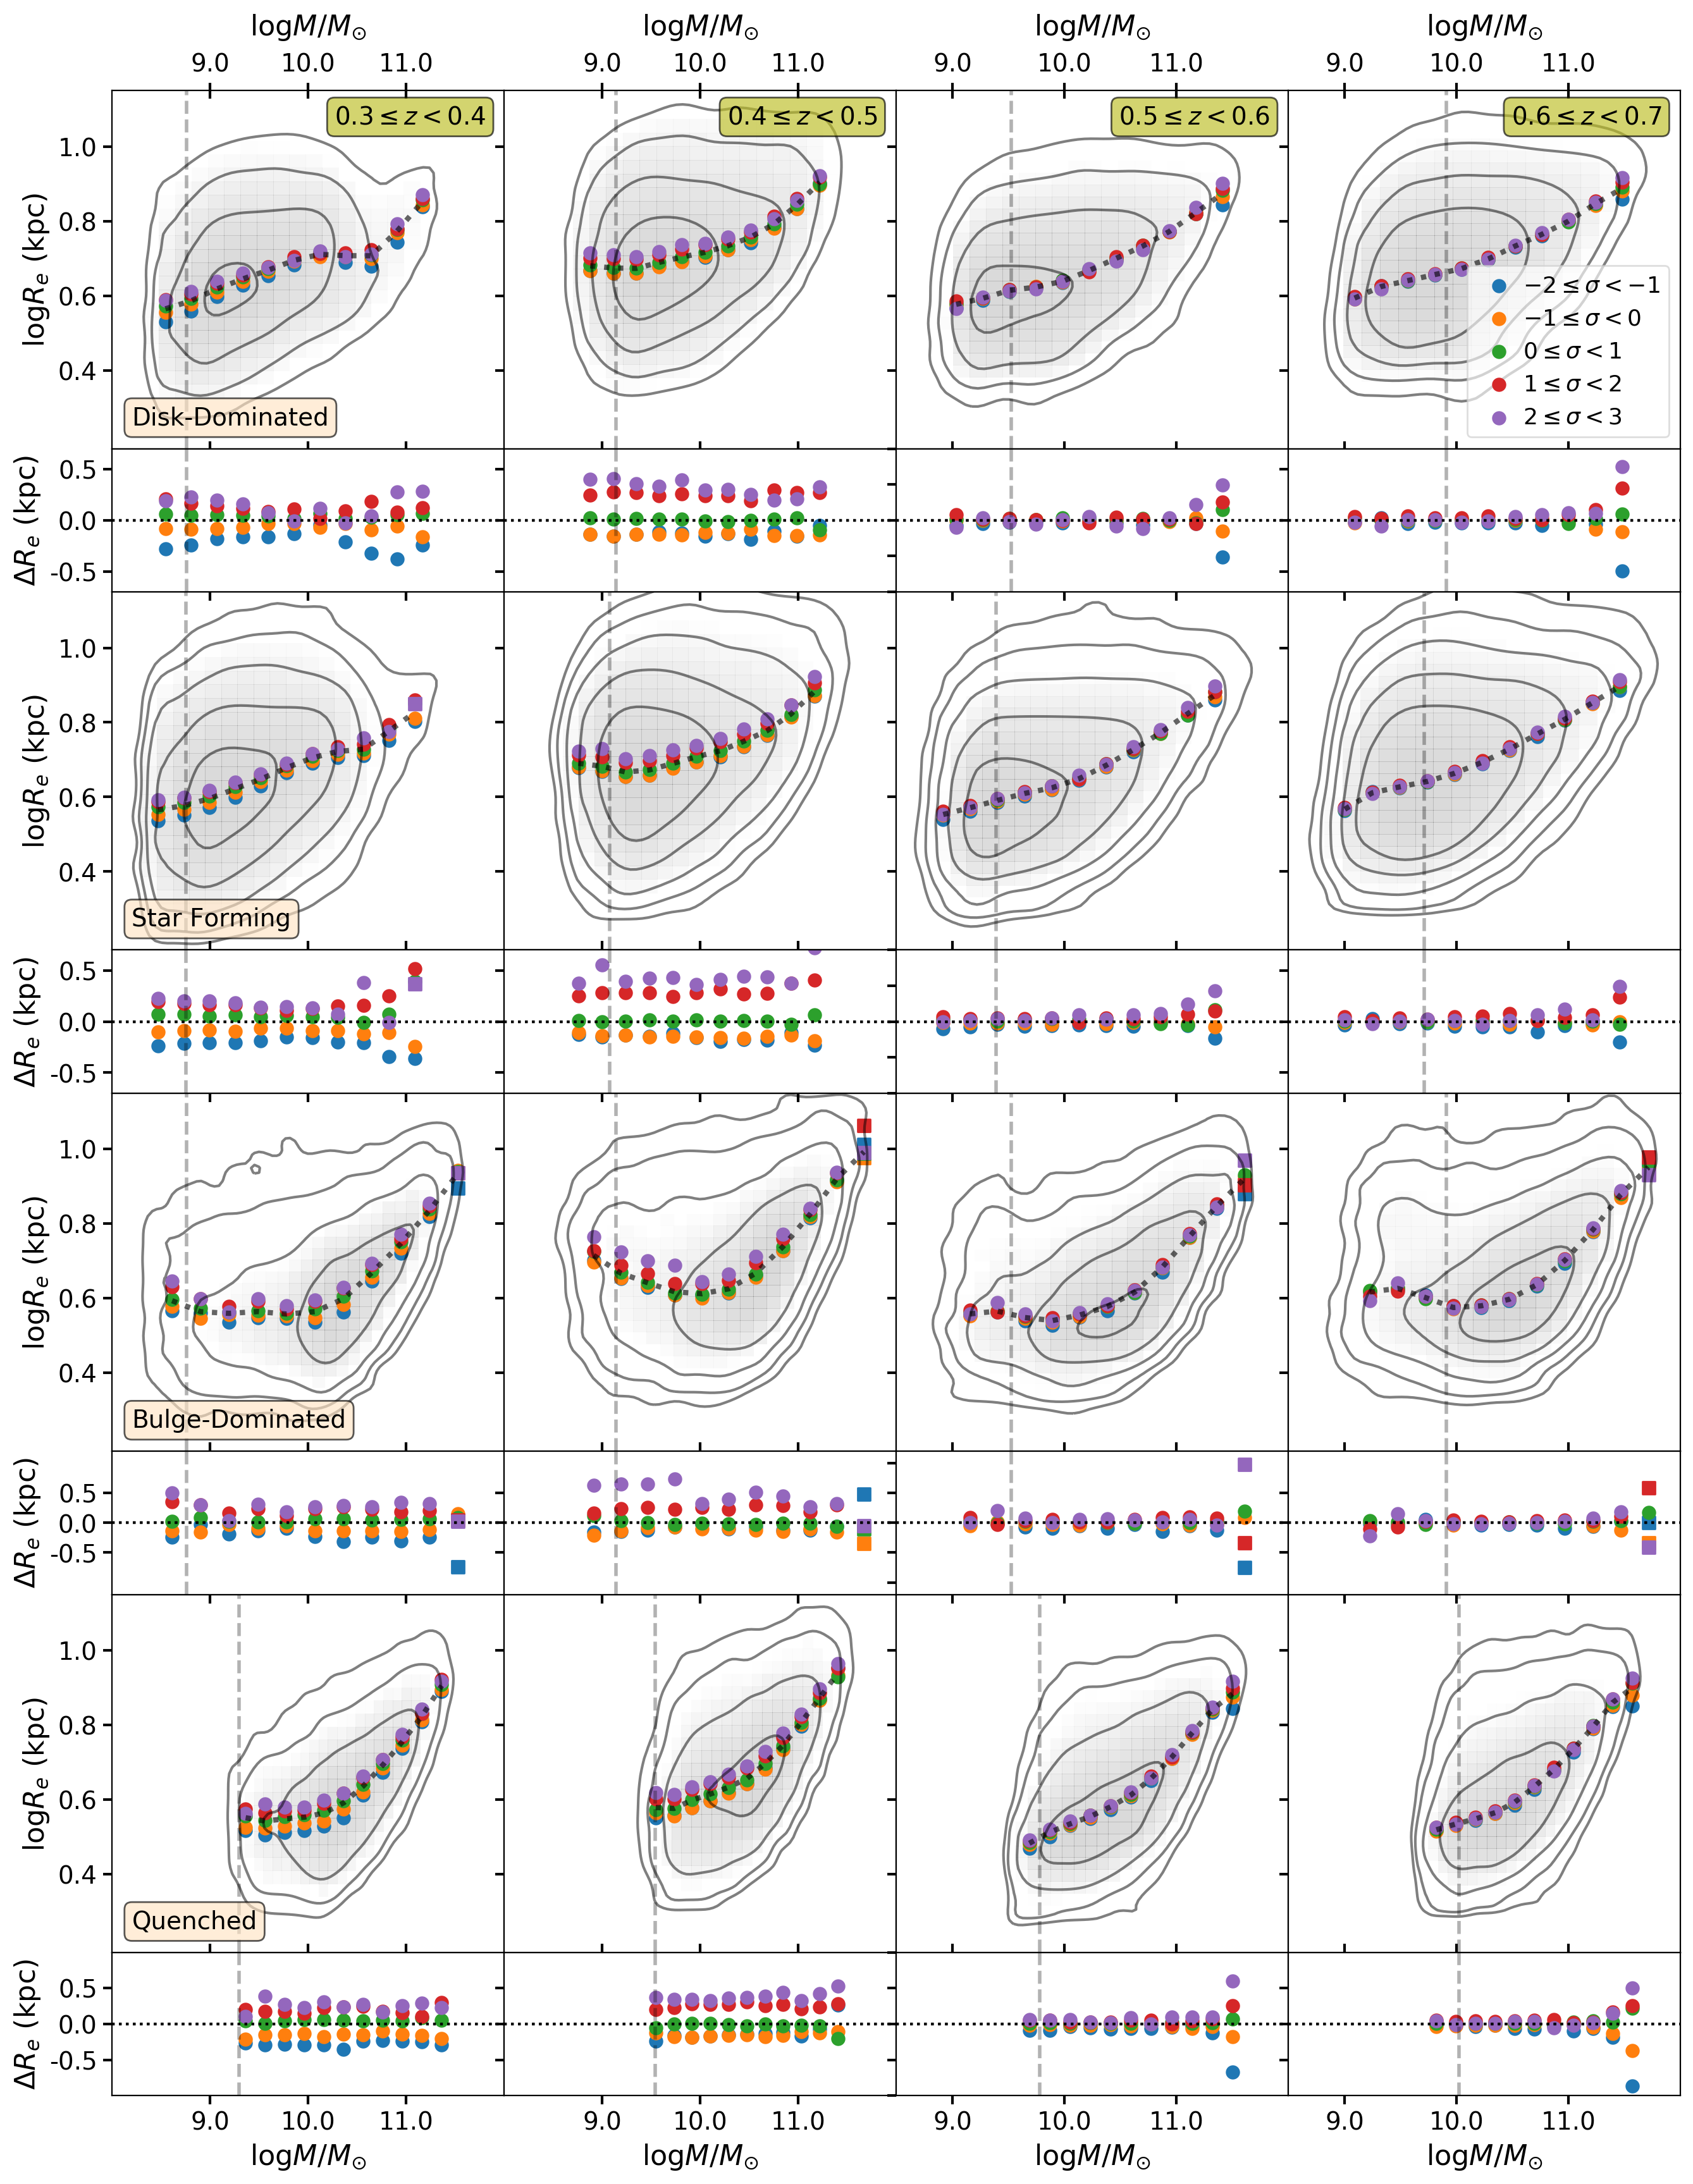
\includegraphics[width = 0.86\textwidth]{r_m_sub.png}
%    \caption{The size-mass relationship shown in the four different redshift slices (different columns) for different sub-samples of galaxies (different rows). The black dotted lines in the upper panels show the median trend; while the colored points show the measurements separately for sub-samples of galaxies in different environments. The bottom panels underneath each contour plot show how the colored points deviate from the overall median trend. The grey dotted vertical line running throughout each panel shows the mass completeness at each redshift bin. Note that some of the color points are squares (instead of circles) --- this indicates that there were less than 100 galaxies in these bins.}
%    \label{fig_c4:r_m_sub}
%\end{figure*}

\begin{figure*}
    \begin{center}
        \subfigure{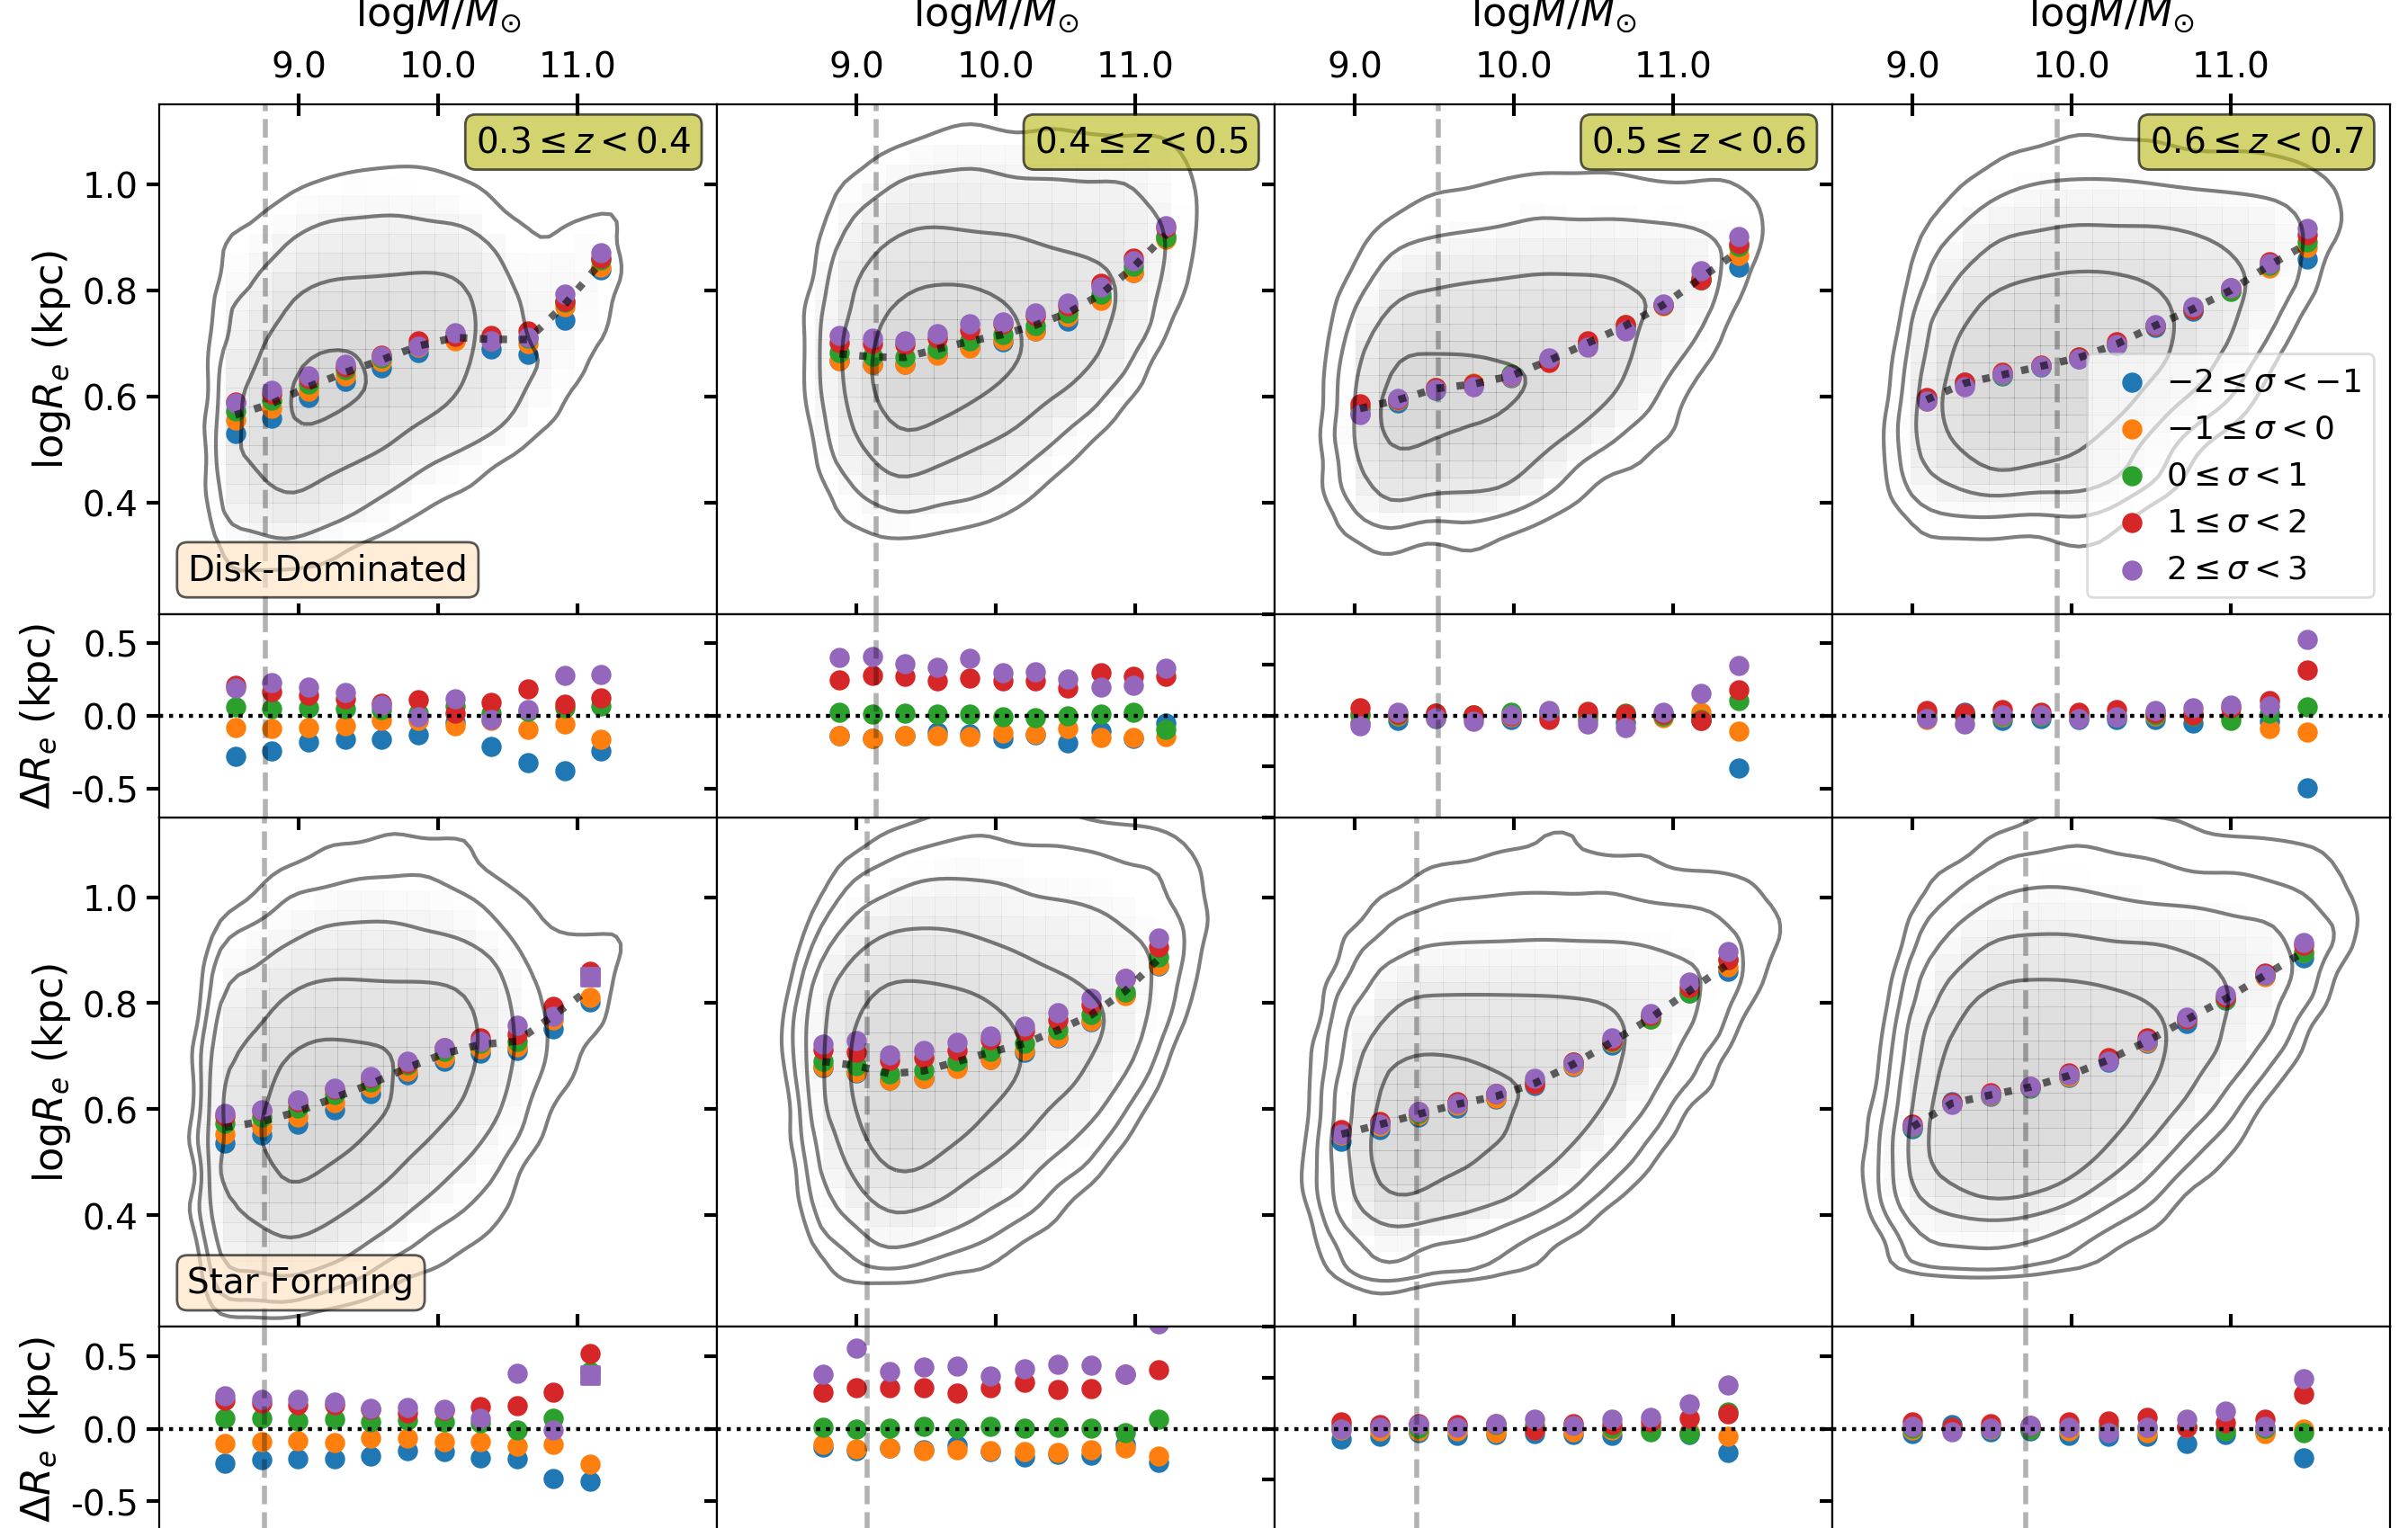
\includegraphics[width=\textwidth]{r_m_sub_1.png}} 
        \subfigure{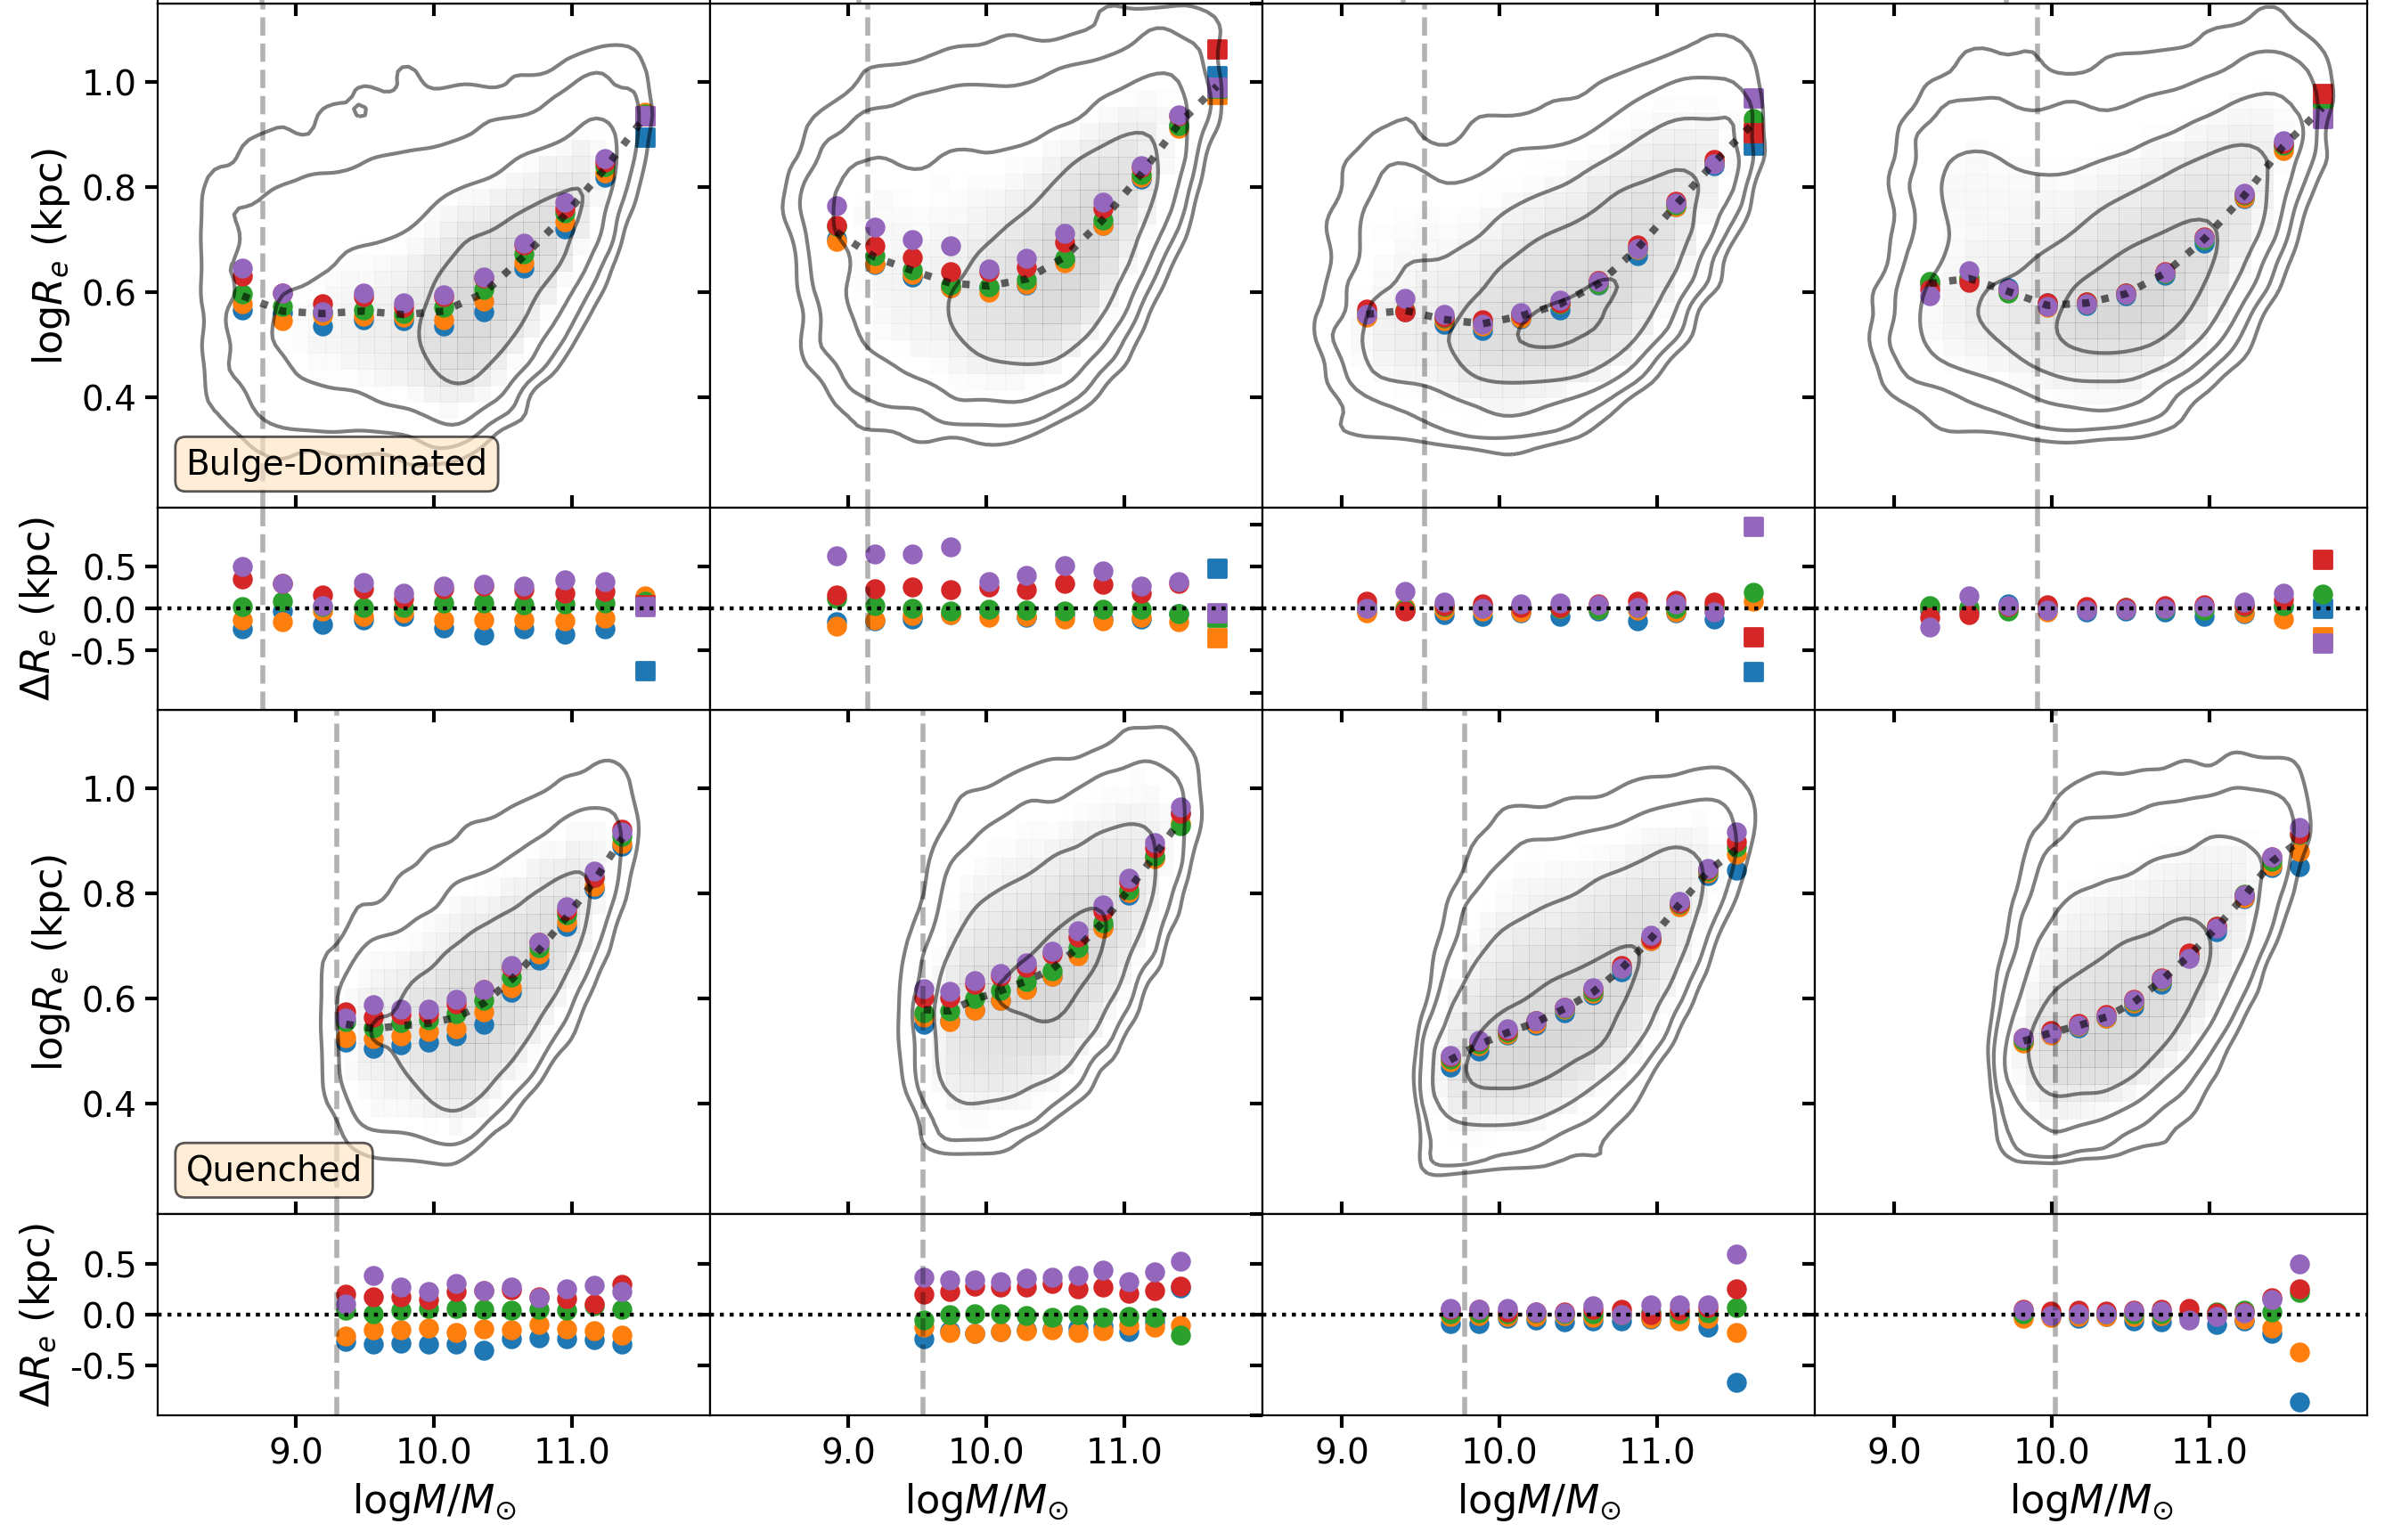
\includegraphics[width=\textwidth]{r_m_sub_2.png}} 
  \end{center}
  \caption{The size-mass relationship shown in the four different redshift slices (different columns) for different sub-samples of galaxies (different rows). The black dotted lines in the upper panels show the median trend; while the colored points show the measurements separately for sub-samples of galaxies in different environments. The bottom panels underneath each contour plot show how the colored points deviate from the overall median trend. The grey dotted vertical line running throughout each panel shows the mass completeness at each redshift bin. Note that some of the color points are squares (instead of circles) --- this indicates that there were less than 100 galaxies in these bins.}
    \label{fig_c4:r_m_sub}
\end{figure*}


In \S \ref{sec_c4:sep_into_subsamples}, we had described how we split our total sample into sub-samples of disk-dominated, bulge-dominated, star-forming, and quiescent galaxies. In this section, we describing the results of running the same analysis that we did in \S \ref{sec_c4:rad_den_all} for each of these sub-populations. The $R_e$ v/s $\sigma_{r=10cMpc}$ plot for each sub-population is shown in Figure \ref{fig_c4:rad_den_sub} and the results of the correlation analysis are reported in Table \ref{tab_c4:corr_subpop_ab}. In order to be concise, we include only order-of-magnitude values in Table \ref{tab_c4:corr_subpop_ab} --- the interested reader can refer to Appendix \ref{sec_c4:ap:corr_coeff} for the un-abridged version of this table. Finally, the size-mass diagram, plotted individually for each sub-population, is available in Figure \ref{fig_c4:r_m_sub}. The format of these figures and table are similar to what was used in the last section for the overall analysis. Note that in this section, we combined the two lower mass bins used in Figure \ref{fig_c4:rad_den_all} and Table \ref{tab_c4:corr_all} into one single bin in order to ensure that we have sufficiently large statistics in each mass bin within each of the four sub-populations.

As can be seen from Table \ref{tab_c4:corr_subpop_ab} and Figure \ref{fig_c4:rad_den_sub}, for the two lower redshift bins, the positive correlation between $R_e$ and $\sigma_{r=10cMpc}$ can be observed for each individual sub-population. For disk-dominated and star-forming galaxies, the effect appears to be marginally stronger in the lower mass bin compared to the higher mass bin. On the other hand, for bulge-dominated and quiescent systems, the effect seems to be marginally stronger at the higher mass end compared to the lower mass end. 

For the two higher redshift bins, the effect is much weaker/absent when compared to the lower redshift bins within each sub-population. However, for bulge-dominated and quiescent systems with $\log M/M_{\odot} > 10.25$, we can confirm the existence of a positive correlation with $>5\sigma$ confidence for both the high redshift bins (refer to Table \ref{tab_c4:corr_subpop_ab}). At the lower mass end for these bulge-dominated and quiescent systems, the effect is either absent or much weaker. For the higher mass star-forming and disk-dominated systems, we can also see the signs of a positive correlation, however the observed statistical significance of the detection is just within the $5\sigma$ confidence threshold and is much weaker compared to the statistical significance observed for the bulge-dominated/quiescent systems.

In line with expectations from previous works \citep[e.g.,][]{mowla19, hsc_mass_size}, Figure \ref{fig_c4:r_m_sub} shows that the steeper slope of the size-mass relation at the higher mass is primarily due to bulge-dominated and quiescent systems. The change in the slope of the power law is significantly less prevalent for disk-dominated and star-forming galaxies. Even when broken down into sub-samples, we don't observe any dependence of the pivotal mass on environmental density.

Figure \ref{fig_c4:r_m_sub} shows the presence of the critical mass of $\sim 10^{11.25}M_{\odot}$ for the $z \geq 0.5$ bins for each individual sub-sample. However, we must note that because of the sample being split up into different groups, using our correlation analysis, we can confirm this result at $>5\sigma$ confidence only for the disk-dominated and the quiescent systems. For the bulge-dominated and star-forming systems, this effect can only be confirmed at $\gtrapprox3\sigma$. It is also interesting to note that for galaxies above the critical mass, the $\Delta R_e$ is significantly higher for bulge-dominated and quiescent systems ($\sim1.2-1.5$ kpc) compared to disk-dominated and star-forming galaxies ($\sim0.6-0.8$ kpc). This is in line with the results seen previously in Table \ref{tab_c4:corr_subpop_ab} and Figure \ref{fig_c4:rad_den_sub}. 

\subsection{Variation of Morphology With Environment} \label{sec_c4:morph_env}

\begin{figure*}[htb]
    \centering
    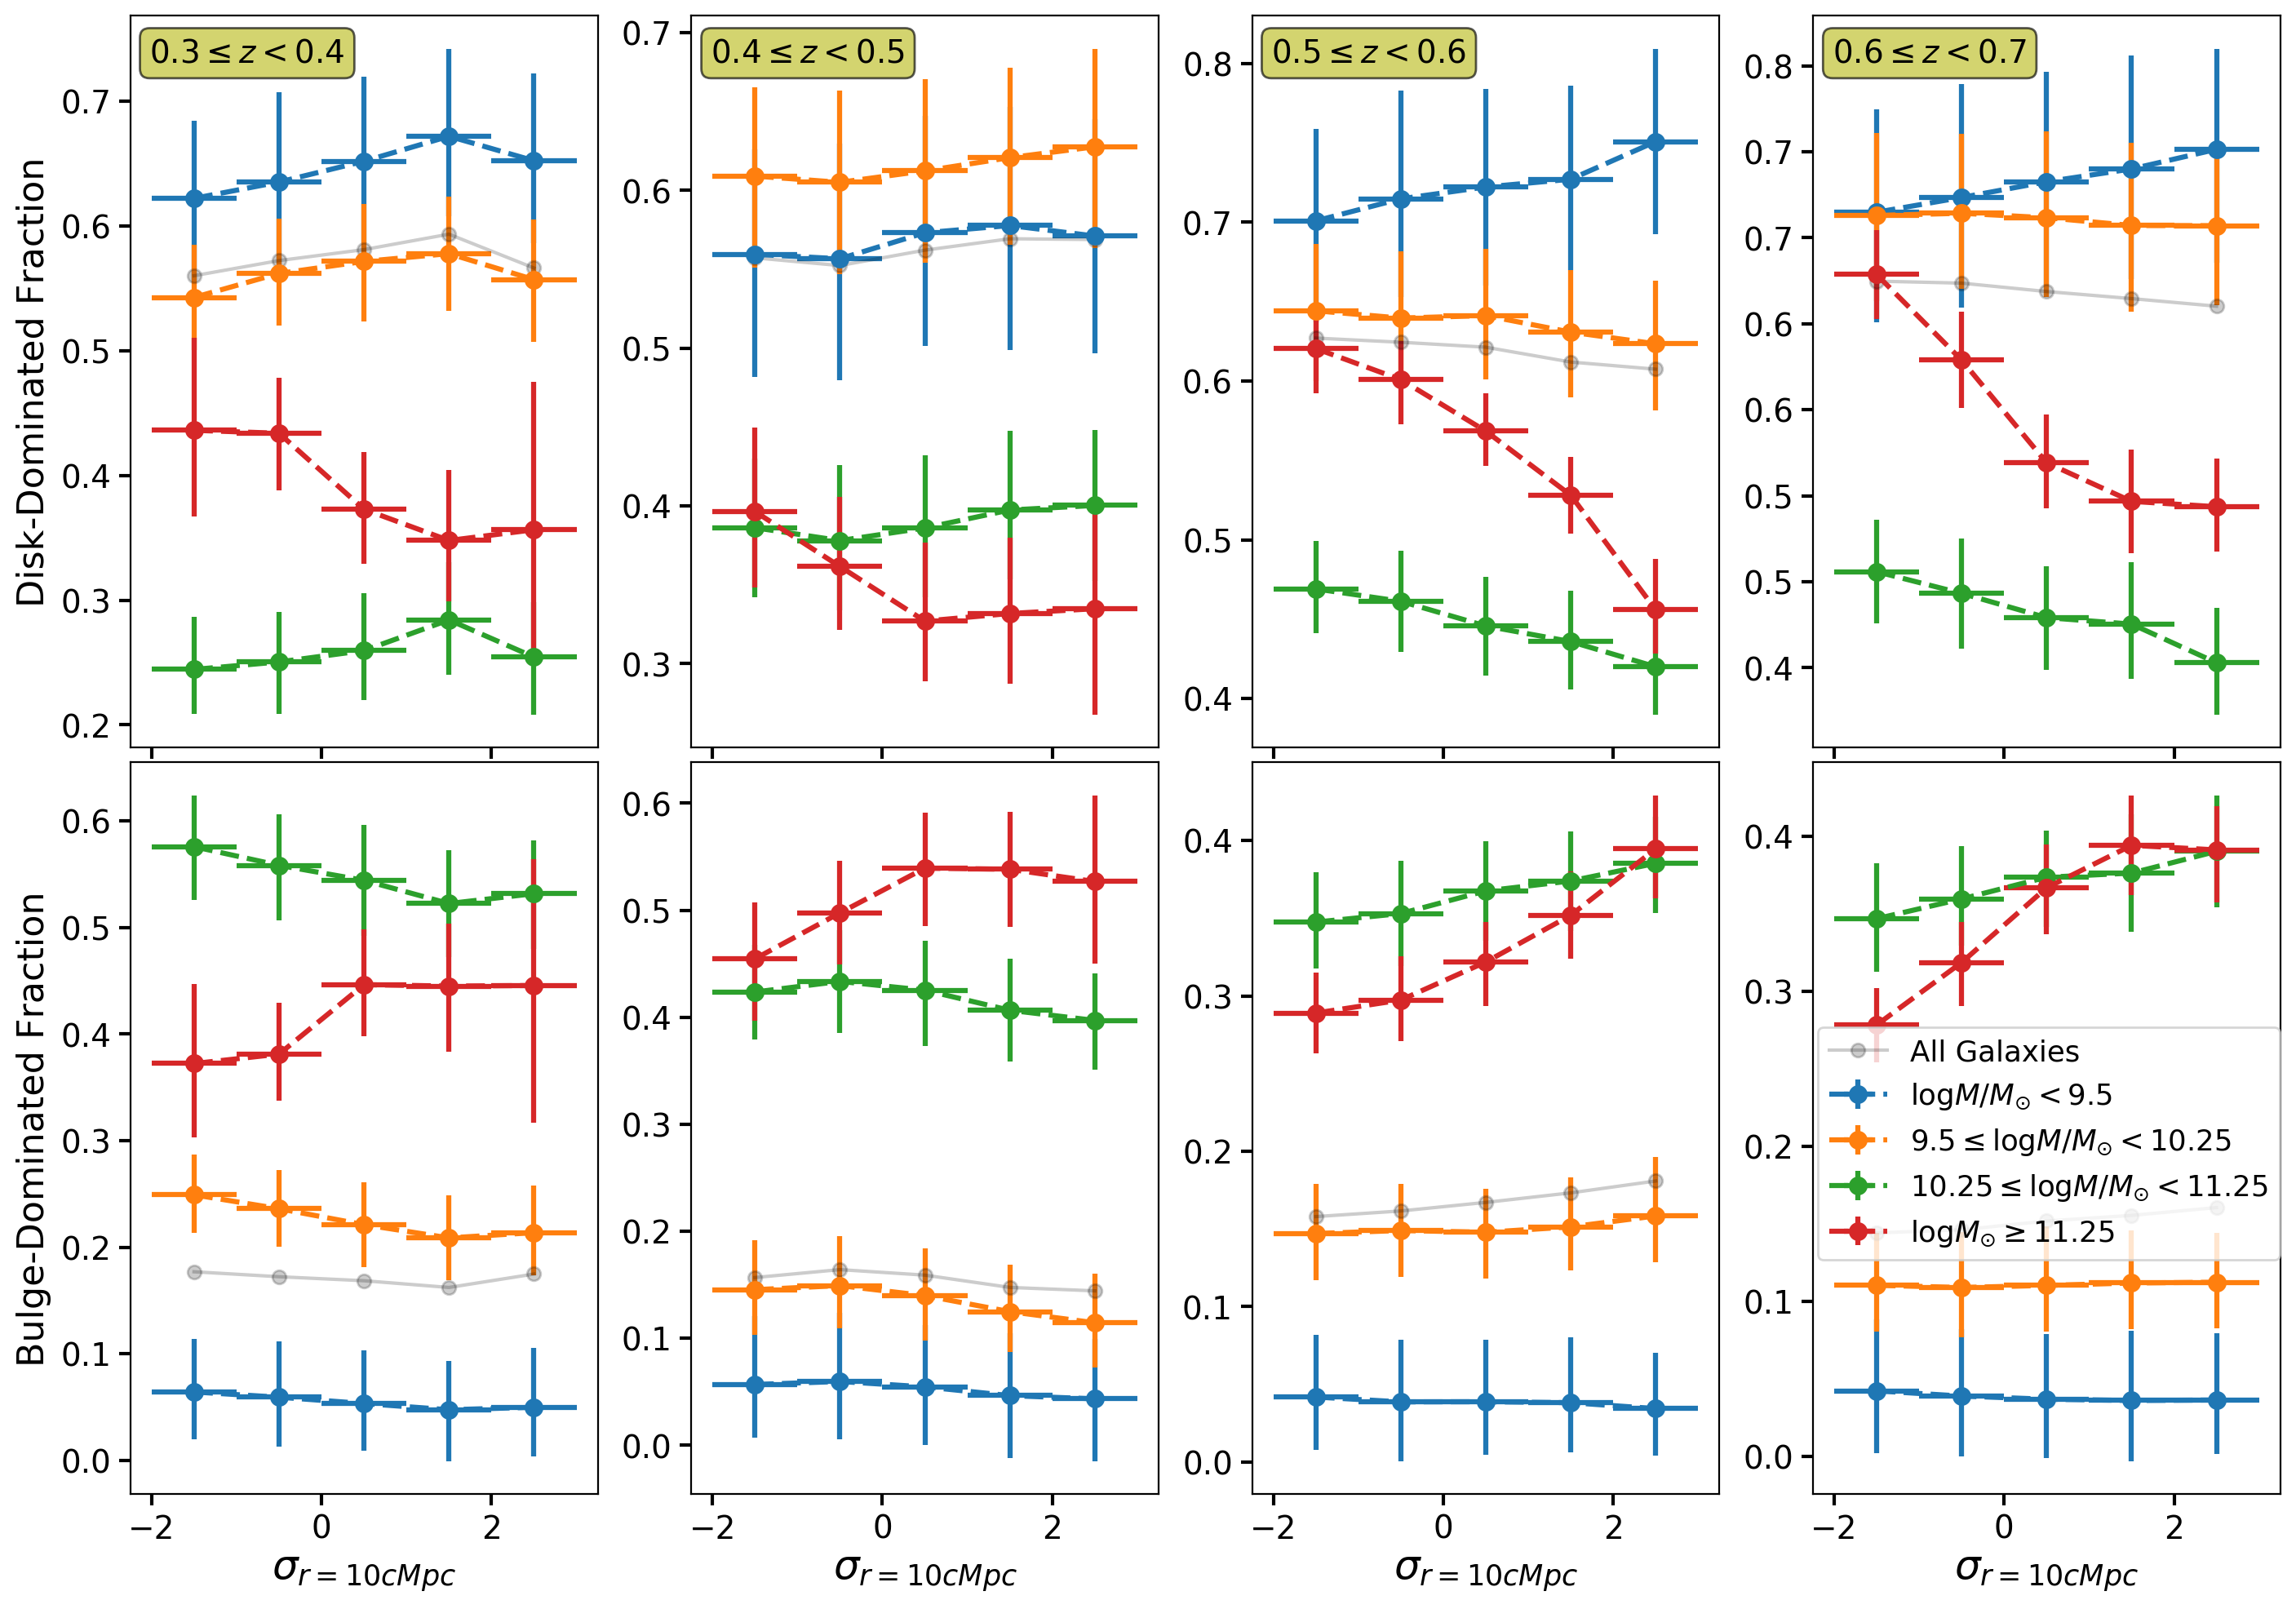
\includegraphics[width = \textwidth]{morph_den.png}
    \caption{The fraction of disk-dominated and bulge-dominated galaxies in bins of different density excess showed for different mass samples. The grey line indicates the overall median trend. The error bars represent the fractional uncertainties taking into account the $68\%$ confidence intervals predicted by \gampen{} on $L_B/L_T$ measurements.}
    \label{fig_c4:morph_den}
\end{figure*}

Having dealt with the variation of $R_e$ with environmental density, we now move to probing how the morphology of galaxies change with environment. \gampen{} predicts the posterior distribution of $L_B/L_T$ for every galaxy and we use the median value of the predicted distribution to split up the galaxies into disk-dominated ($L_B/L_T < 0.4$) and bulge-dominated fractions ($L_B/L_T > 0.6$). We then study how these fractions are varying as a function of $\sigma_{r=10cMPc}$.

Figure \ref{fig_c4:morph_den} shows how the measured fractions vary for four different mass-bins within each redshift slice. In order to estimate the error bars shown in Figure \ref{fig_c4:morph_den}, we sampled values of $L_B/L_T$ 1000 times for each galaxy from the predicted posterior distribution. Thereafter, we measured the bulge and disk-dominated fractions for each of these 1000 draws and the error bars shown in Figure \ref{fig_c4:morph_den} represent the $68\%$ confidence interval of the distribution of disk- and bulge-dominated fractions. 

We would like to note here that, as described above, our morphological classification is based on $L_B/L_T$. Thus the disk-dominated / bulge-dominated fractions measured above are not expected to completely correlate with measurements of ``early-type" and "late-type" morphological fractions identified using visual inspection or machine learning frameworks. Therefore, the following results should be interpreted as such in their own right.

%Note that here we can perform our correlation analysis only on binned data; unlike \S \ref{sec_c4:rad_den}, where we used every single galaxy on its own. XXXXXXXXXXX 

We find that for the highest mass bin ($\log M/M_{\odot} > 11.25$), the fraction of bulge-dominated galaxies increases in denser environments, while the fraction of disk-dominated galaxies drops in-tandem. We observe this effect in all four redshift bins, although the result is marginally more statistically significant and stronger in the higher two redshift bins. 

The second highest mass bin ($10.25 \leq \log M/M_{\odot} < 11.25$ ) also displays a similar trend in the higher two redshift bins. The effect is absent/less statistically significant in the lower redshift bins. For the lowest two mass bins, we cannot identify any statistically significant trend in any redshift slice. 


\section{Discussion \& Summary} \label{sec_c4:discussion}

In this section we, summarize what we find in \S \ref{sec_c4:results}; and reflect on possible explanations for the correlations we observe. 

\subsection{Summary of Observed Correlations} \label{sec_c4:summary}

For $0.3 \leq z < 0.5$:-

\begin{itemize}
    \item We can confirm with $>5 \sigma$ confidence that galaxies in denser environments are larger than their counterparts with similar masses in less-dense environments. 
    \begin{itemize}
        \item The above result holds true for the entire mass-range probed in this study. We cannot detect any significant monotonic change in the strength of the correlation with mass (see lower panel of Figure \ref{fig_c4:r_m_all}). 
        \item However, the effect does appear to be marginally stronger in the highest mass-bin we use (see $\alpha$ and $p$ in Table \ref{tab_c4:corr_all}).
    \end{itemize}
    \item The positive correlation between $R_e$ and denser environments also holds true individually for disk-dominated, bulge-dominated, star-forming, and quiescent sub-populations drawn from our total sample. 
    \begin{itemize}
        \item The above result also holds true for entire mass-range probed in this study and we cannot detect any significant monotonic change in the strength of the correlation with mass (see lower panel of Figure \ref{fig_c4:r_m_sub}).
        \item However, the effect does appear to be marginally stronger in the lower mass-bin for disk-dominated and star-forming galaxies (see $\alpha$ and $p$ in Table \ref{tab_c4:corr_subpop_ab}).
    \end{itemize}  
    \item For galaxies with $\log M/M_\odot > 10.25$, the bulge-dominated fraction of galaxies grows in denser environments at the expense of the fraction of disk-dominated galaxies. For lower mass bins, we observe no/marginal trends, when considering the errors on our fraction measurements.
\end{itemize}

For $0.5 \leq z < 0.7$:-
\begin{itemize}
    \item The overall positive trend between galaxy radius and large-scale structural density is much weaker/negligible when compared to the lower redshifts. 
    \begin{itemize}
        \item For $0.6 \leq z < 0.7$, we cannot detect any statistically significant correlation, while for $0.5 \leq z < 0.6$, we detect a weak positive correlation. 
        \item However, there appears to be a critical stellar mass ($\sim2\times10^{11} M_\odot$) above which there is a strong preference for galaxies in denser environments to be larger. Although at the tail end of the mass distribution, we have enough statistics to confirm this effect $>5\sigma$ confidence. 
    \end{itemize}
    \item When the sample is divided into disk-dominated, star-forming, bulge-dominated, and quiescent galaxies:- we correspondingly find that the overall positive correlation seen at lower z disappears/weakens when compared within each sub-population.
    \begin{itemize}
        \item However, for $\log M/M_{\odot} > 10.25$ bulge-dominated and quiescent galaxies, we can detect a positive correlation with $>5\sigma$ for both the higher redshift bins. This effect weakens/disappears in the lower mass bin. 
        \item For $\log M/M_{\odot} > 10.25$ star-forming and disk-dominated galaxies, we can also see signs of a positive correlation; however the observed correlation and its statistical significance is much weaker compared to the bulge-dominated/quiescent galaxies mentioned above. 
        \item The existence of the previously mentioned critical stellar mass ($\sim2\times10^{11} M_\odot$) can be observed for each sub-population, above which we can observe a clear correlation of radius and environmental density. This observed correlation above the critical stellar mass is stronger for bulge-dominated and quiescent systems compared to disk-dominated and star-forming systems. 
    \end{itemize}
    \item For galaxies with $\log M/M_\odot > 10.25$,  the bulge-dominated fraction of galaxies grow in denser environments at the expense of disk-dominated galaxies. For lower mass bins, we observe no/marginal trends, when considering the errors on our fraction measurements.
\end{itemize}

\subsection{Comparison to Past Studies} \label{sec_c4:comp}

The correlations noted in \S \ref{sec_c4:summary} in part help explain the conflicting results observed previously, as outlined in Table \ref{tab_c4:lit_survey}. As our results clearly show, galaxy radius is primarily set by stellar mass, and therefore, to observe the secondary dependence of radius on environment, it is imperative to have a large sample in order to achieve statistically significant results. 

All the studies noted in Table \ref{tab_c4:lit_survey} are smaller in sample size by a factor of $\sim100-10,000$ compared to this work. Additionally, none of the studies previously mentioned:- a) used an end-to-end Bayesian framework like \gampen{} and therefore had no robust handle on the amount of uncertainty in their $R_e$ measurement\footnote{as shown in \citet{hsc_wide_morphs}, light profile fitting tools significantly underestimate uncertainties}; b) incorporated their $R_e$ errors into the correlation analysis in a statistically robust way.

Therefore, given the low value of the observed correlation co-efficient and its dependence on redshift, stellar mass, morphology, and star-formation; it is not surprising that previous studies observed the variety of correlation shown in Table \ref{tab_c4:lit_survey}. In fact, if we restrict our total sample size to $\sim1000$ galaxies and repeat our analysis without taking into account $R_e$ errors, we cannot reproduce our own results with high statistical significance. In fact, we observe significantly varying trends, with every different sampling from all the galaxies and the $R_e$ distribution of each galaxy.

Some of the previous studies probing $z > 0.5$ redshifts have observed the correlation only for passive/quiescent/early-type galaxies \citep[e.g.,][]{Cooper12,Lani13,Bassett13}. This is in agreement with the fact that in our study at $z > 0.5$, the statistical significance of the observed correlation is much stronger for higher mass quiescent and bulge-dominated galaxies. Additionally, \cite[e.g.,][]{Afonso19} observed the correlation only for galaxies with $\log M/M_{\odot} > 11$. This almost perfectly coincides with the critical threshold stellar mass that we observe for $z > 0.5$. 

\subsection{Possible Explanations of Observed Correlation} \label{sec_c4:theory}
Given our current understanding of the hierarchical galaxy formation model in the $\Lambda$ cold dark matter ($\Lambda$CDM) universe, galaxy sizes are affected by a host of different factors. In order to understand the reason behind the correlations with large scale structure that we observe in this work, comprehensive follow up work is needed using N-body and cosmological simulations. However, given the existing body of literature, it is possible to isolate a few causes for the correlations we observed in \S \ref{sec_c4:results}.

Classic models of galaxy formation \citep{fall80,mo98} based the radial sizes of galaxies on the spin of their dark matter halos, and predicted that galaxy sizes should be proportional to the spin and size of the halo. Since then, there have been several follow-up studies using the standard abundance matching model in N-body simulations as well as in zoom-in hydro-cosmological simulations \citep[e.g.,][]{Kravtsov13, somerville18, jiang19}, all of which have converged on the general prediction

\begin{equation}
    R_e = A R_{vir}
    \label{eq:r_e_vir}
\end{equation}

although predicted nature of A has been varied. Different studies have predicted A to be either constant or dependant on halo concentration and/or halo spin. We refer to an interested reader to \citet{wechsler_tinker} for an extended discussion.

It is well known that in the $\Lambda$CDM paradigm, the clustering of dark matter halos depend on various halo properties other than mass \citep[e.g.,][]{wechsler02,wechsler06,gao07} -- this is commonly referred to as `assembly bias' (see \citet{mao18} for a recent overview). As a consequence of this effect larger halos (of the same mass) typically reside in more denser environments, and  halos (of the same mass) with higher concentration and spin are known to cluster more strongly. 

Therefore, it can be expected from Equation \ref{eq:r_e_vir}, that galaxies in denser environments will be preferentially larger when compared to equally massive counterparts in less-dense environments. We posit that this effect is resulting in the positive correlations between $R_e$ and $\sigma_{r=10cMPc}$ that we observe in \S \ref{sec_c4:results}. The fact that Equation \ref{eq:r_e_vir} has been found to hold true for almost all morphological types and across a wide range of stellar masses \cite[e.g.,][]{Kravtsov13} could explain why we see the effect (at lower z) for all mass ranges and for all sub-populations of galaxies. 

\citet{somerville18} found the ratio between stellar-radius to halo-radius ratio (A) to be only weakly dependant on mass; and reported that A increases by a factor of 1.5 from $z\sim3$ to $z\sim0.4$ for galaxies with $\log M/M_{\odot} \gtrapprox 10$. This is consistent with what we find:- overall, we find that the strength of the correlation between $R_e$ and $\sigma_{r=10cMPc}$ to be weakly dependant on mass and stronger at lower redshifts. 

The fact that we observe a stronger correlation for massive bulge-dominated and quiescent systems can be understood from the perspective of the correlation between size-growth in these systems and mergers. It has been proposed by many that for bulge-dominated/quiescent systems, size-growth at higher masses is dominated by minor, dry mergers \citep[e.g.,][]{shankar13} and the same conclusion has also been drawn from observational results \citep[e.g.,][]{mowla19,hsc_mass_size}. Given that mergers are more efficient and frequent in denser environments, bulge-dominated/quiescent systems in dense environments undergo a more rapid size evolution compared to their equally massive counterparts in lower density environments --- resulting in larger quiescent galaxies in denser environments. The fact that the observed increased correlation for bulge-dominated/quiescent systems is mostly observed in the higher redshift bins could be due to the fact that mergers are though to be more prevalent at higher redshifts. Since size growth at lower masses and for disk-dominated/star-forming systems are not dominated by mergers, it is not surprising that our observed correlation is weaker/absent for these cases. 

Mergers can also be evoked to explain the redshift evolution of the correlation observed for the entire sample. Given that as time progresses, at lower redshifts, galaxies become more gas poor and galaxies closer to the present epoch are preferentially born from a series of gas-poor mergers. Given the positive correlation between merger rate and efficiency with environment, this could in part explain why we see a stronger correlation at lower redshifts. 

The trend that we observe between galaxy morphology and environmental density in Figure \ref{fig_c4:morph_den} is largely consistent with what has been observed previously. We posit that the results indicate that the transformation of (star-forming) disk-dominated galaxies into (quiescent) bulge-dominated galaxies occur at an accelerated rate in denser environments. Given that various effects responsible for such a transformation (e.g., mergers, ram pressure stripping, gas strangulation) are more prevalent in denser environment, it is not surprising that we observe the rate of morphological transformation to be more in denser regions. The fact that we do not observe this correlation at lower masses can be due to two reasons:- i) massive galaxies are more likely to experience mergers compared to less massive galaxies; ii) determining $L_B/L_T$ is more difficult for smaller less-massive galaxies, which leads to bigger error bars at these lower masses (see blue and orange lines in top panel of Figure \ref{fig_c4:morph_den}).



\section*{Chapter Acknowledgments}

CMU and AG would like to acknowledge support from the National Aeronautics and Space Administration via ADAP Grant 80NSSC18K0418. 

AG would like to acknowledge the support received from the Yale Graduate School of Arts \& Sciences through the Dean's Emerging Scholars Research Award.

AG would like to acknowledge helpful discussions with Kaustav Mitra. 

The Hyper Suprime-Cam (HSC) collaboration includes the astronomical communities of Japan and Taiwan, and Princeton University. The HSC instrumentation and software were developed by the National Astronomical Observatory of Japan (NAOJ), the Kavli Institute for the Physics and Mathematics of the Universe (Kavli IPMU), the University of Tokyo, the High Energy Accelerator Research Organization (KEK), the Academia Sinica Institute for Astronomy and Astrophysics in Taiwan (ASIAA), and Princeton University. Funding was contributed by the FIRST program from Japanese Cabinet Office, the Ministry of Education, Culture, Sports, Science and Technology (MEXT), the Japan Society for the Promotion of Science (JSPS), Japan Science and Technology Agency (JST), the Toray Science Foundation, NAOJ, Kavli IPMU, KEK, ASIAA, and Princeton University. 

This paper makes use of software developed for the Large Synoptic Survey Telescope. We thank the LSST Project for making their code available as free software at  \href{http://dm.lsst.org}{http://dm.lsst.org}.

The Pan-STARRS1 Surveys (PS1) have been made possible through contributions of the Institute for Astronomy, the University of Hawaii, the Pan-STARRS Project Office, the Max-Planck Society and its participating institutes, the Max Planck Institute for Astronomy, Heidelberg and the Max Planck Institute for Extraterrestrial Physics, Garching, The Johns Hopkins University, Durham University, the University of Edinburgh, Queen’s University Belfast, the Harvard-Smithsonian Center for Astrophysics, the Las Cumbres Observatory Global Telescope Network Incorporated, the National Central University of Taiwan, the Space Telescope Science Institute, the National Aeronautics and Space Administration under Grant No. NNX08AR22G issued through the Planetary Science Division of the NASA Science Mission Directorate, the National Science Foundation under Grant No. AST-1238877, the University of Maryland, and Eotvos Lorand University (ELTE) and the Los Alamos National Laboratory.

Based, in part, on data collected at the Subaru Telescope and retrieved from the HSC data archive system, which is operated by Subaru Telescope and Astronomy Data Center at National Astronomical Observatory of Japan.




